
\documentclass[11pt, a4paper,titlepage]{article}
\usepackage[spanish, es-tabla, es-nodecimaldot]{babel}
\selectlanguage{spanish}
%% NO AGREGAR PAQUETES ANTES DE BABEL!


%%%%%%%%%%%%%%%%%
% DOCUMENT FONT %
%%%%%%%%%%%%%%%%%
\usepackage[T1]{fontenc}
\usepackage[utopia]{mathdesign}
%\newcommand{\gtrsim}{\text{ mayor o parecido a }}

%%%%%%%%%%%%%%%
% PAGE FORMAT %
%%%%%%%%%%%%%%%
\usepackage[a4paper,top=1.5cm,bottom=1.5cm,left=2cm,right=2cm]{geometry}
\setlength{\parindent}{10pt} %Sangria al comienzo de un paragraph
%%----------------------------------------------------

%%%%%%%%%%%%%%%%%%%
% GENERAL PURPOSE %
%%%%%%%%%%%%%%%%%%%
\usepackage[
hyperfootnotes=false,
urlcolor=blue,
colorlinks=true,
citecolor=red]{hyperref}
%\usepackage{units} % permite usar nicefrac
\usepackage{graphicx,xcolor,caption,subcaption,multirow}
\usepackage{amsmath,array}

%%%%%%%%%%%%%%%%
% BIBLIOGRAPHY %
%%%%%%%%%%%%%%%%
\usepackage{natbib}
\bibliographystyle{unsrtnat}

%%%%%%%%%%%%%
% FOOTNOTES %
%%%%%%%%%%%%%
\usepackage[symbol,perpage]{footmisc}
\renewcommand*{\thefootnote}{\fnsymbol{footnote}}
\let\oldpart\part

\renewcommand{\part}[1]{\clearpage \oldpart{#1}}

%\usepackage{bigfoot} % to allow verbatim in footnote
\usepackage[numbered,framed]{matlab-prettifier}

\let\ph\mlplaceholder % shorter macro
\lstMakeShortInline"
\renewcommand{\lstlistingname}{Código}
\renewcommand{\lstlistlistingname }{Códigos \Matlab}
\lstset{
  style              = Matlab-editor,
  basicstyle         = \mlttfamily,
  escapechar         = ",
  mlshowsectionrules = true,
  numbers = none,
  tabsize=4,
  literate = {-}{-}1,
}

\begin{document} 

\pagestyle{empty}
\begin{titlepage} %Esta es la caratula
	
\centering
{Instituto Tecnológico de Buenos Aires \par}
\vspace{2cm}

{\scshape \Huge \bf Elementos Finitos\par}

\vspace{.8cm}

{\scshape\Large Apunte no oficial para la materia 30.07 y 31.92 \par}
\vfill
\vspace{3cm}

{
	\centering
	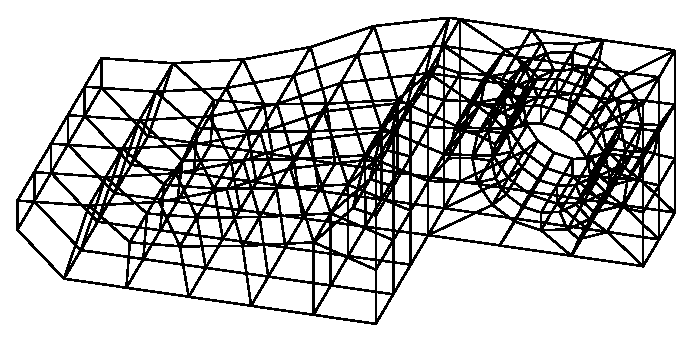
\includegraphics[width=\textwidth]{fig/sear.eps}
	
}
\vfill

{\scshape\Large\textbf{Patricio Whittingslow} \par}
\vspace{4cm}
\medskip %medskip,smallskip,vspace son todos comandos para dejar espacio en blanco entre cosas

\end{titlepage} %Termina la caratula
\pagestyle{plain}

\tableofcontents
\vspace{1cm}
Este documento fue creado usando \LaTeX{} para las materias Elementos Finitos I y Elementos Finitos II del ITBA por un alumno. Edición \today.

El código fuente se puede encontrar mi repositorio de github \href{https://github.com/soypat/whittileaks}{~/soypat/whittileaks}. Licensiado bajo Creative Commons 4.0 CC-BY-NC-SA.

License: \href{https://creativecommons.org/licenses/by-nc-sa/4.0/}{Attribution-NonCommercial-ShareAlike 4.0 International.} 
\lstlistoflistings

\clearpage

\pagestyle{plain}
\setcounter{page}{1}
\setcounter{section}{-1}
\section{Introducción al Método de los Elementos Finitos}
El análisis o método de elementos finitos (FEA por \textit{finite element analysis}) es usado para obtener una solución numérica de un problema de campo (electrostático, térmico, tensiones). Matemáticamente estos problemas están definidos como ecuaciones diferenciales o como un integral. Ambas expresiones pueden formularse con elementos finitos.

Las ventajas de FEA son
\vspace{-.3cm}
\begin{itemize}
	\item Es aplicable a cualquier problema de campo
	\item No hay restricciones geométricas
	\item No hay restricciones al tipo de cargas o condiciones de borde que se pueden aplicar
	\item Se puede formular para materiales que no son isotrópicos e incluso el tipo de material puede cambiar dentro de un elemento
	\item Se pueden combinar distintos tipos de elementos en un modelos, por ejemplo, unir barras con vigas o incluso con elementos 3D.
	\item La aproximación se puede mejorar fácilmente refinando la malla donde hay gradientes de tensión altos
\end{itemize}
\vspace{-.7cm}
\subsection*{Proceso de resolución}
El primer paso es identificar y \textbf{clasificar} el problema.
\begin{itemize}
	\item Cuales son los fenómenos físicos involucrados y que resultados se buscan del análisis
	\item Depende del tiempo? (estático o dinámico)
	\item Hace falta una resolución iterativa? (no linealidad: radiación, plasticidad)
\end{itemize} 

Luego se comienza el \textbf{modelado} del problema.
\begin{itemize}
	\item Se excluyen los detalles superfluos, dejando los esencial para describir el problema con un margen de error adecuado sin complicar las cosas innecesariamente 
	\item Un \textit{modelo geométrico} se convierte en un \textit{modelo matemático} cuando se describe su comportamiento mediante ecuaciones diferenciales y condiciones de borde.\footnote{Un modelo de FEA no es la realidad, es una \textit{simulación}. Difícilmente se obtengan resultados buenos cuando se aplique FEA a un modelo matemático que no refleja la realidad de forma apropiada.}
	\end{itemize}
Un modelo matemático es una idealización donde se simplifican la geometría, propiedades del material, cargas y/o condiciones de borde en base del entendimiento del analista acerca lo que tiene (o no) importancia al momento de obtener los resultados requeridos.


Finalmente llega el momento de la \textbf{discretización}. Un modelo matemático se discretiza dividiéndolo en una malla de elementos finitos. De esta forma, un campo continuo es representado como una función partida la cual es definida por una cantidad finita de variables nodales e interpolación dentro de cada elemento.
\vspace{-.4cm}
\subsection*{Tipos de error}
Al momento de discretizar se introduce error conocido como \textbf{error de discretización}. Eso sucede porque se aproxima un campo \textit{suave} con una función partida. Aumentar el numero de elementos puede disminuir este error pero nunca eliminarlo.

Aún reduciendo el error de discretización se tendría \textbf{error numérico} porque toda computadora usa números de finita precisión para efectuar aritmética. Este error suele ser mínimo cuando se discretiza de forma adecuada y no se tiene una situación física propensa al \textit{mal condicionamiento}.

Cabe destacar que se introdujo error antes de hacer una sola cuenta! El \textbf{error de modelado} se introduce por necesidad de simplificar el problema. Las cargas puntuales, los soportes fijos y los materiales perfectamente homogéneos no existen en la realidad! \cite{cook2007concepts}.

\subsection*{Principios básicos de elementos finitos}

La ecuación que se resuelve es
\[
M\ddot{d} + C\dot{d} + Kd = F^{\mathrm{externas}}
\]
para un sistema mecánico. Es común tratar problemas estáticos tener como variables de entrada las fuerzas externas $F^{\mathrm{externas}}$ (peso propio, fuerzas aplicadas, fuerza centrifuga etc.) y la rigidez del sistema $K$. Los desplazamientos $d$ sería la variable que se desea obtener. La ecuación a resolver entonces es
\[
d =K^{-1} \cdot F^{\mathrm{externas}}
\]

El método de los elementos finitos entonces tiene su campo de rigidez $K$ que se suele llamar la matriz de rigidez global $\MK$. Esta asocia rigidez con los grados de libertad de los nodos obtenidos de la discretización. Para cuerpos sólidos en el espacio hay 6 grados de libertad, 3 de desplazamiento ($u$, $v$ ,$w$) y tres de giro ($\varphi$, $\theta$, $\psi$). 

Antes de discretizar un modelo se eligen las direcciones $x$, $y$, $z$ globales. Los desplazamientos obtenidos corresponderán a estas direcciones.

\part{Programación del método de los elementos finitos}

\newcommand{\Numberof}{N}
\newcommand{\Numberlocal}{n}
\newcommand{\DOF}{\vartheta}
\newcommand{\Nnod}{\ensuremath{\Numberof_{\mathrm{nod.}}}}
\newcommand{\Ndims}{\ensuremath{\Numberof_{\mathrm{dim.}}}}
\newcommand{\Nelem}{\ensuremath{\Numberof_{\mathrm{elem.}}}}
\newcommand{\Ndofpornod}{\ensuremath{\DOF_{\mathrm{nod.}}}}
\newcommand{\Ndof}{\ensuremath{\Numberof_{\mathrm{dof}}}}

\newcommand{\Nnodporelem}{\ensuremath{\Numberlocal_{\mathrm{nod.}}}}
\newcommand{\Ndofporelem}{\ensuremath{\Numberlocal_{\mathrm{dof}}}}

\begin{table}[htb!]
	\centering
	\begin{tabular}{ccl}
		Objeto matemático & Nombre de variable & Definición \\ \hline
	\Nnod	& \texttt{Nnod}                   &    Número de nodos        \\
	\Nelem	& \texttt{Nelem}                   &    Número de elementos       \\
	\Ndofpornod	& \texttt{Ndofpornod}                   &    Número dof por nodo       \\
	$\Ndof=\Ndofpornod \cdot \Nnod$	& \texttt{Ndof} {\footnotesize{}o simplemente} \texttt{dof}                   &    Número de dof        \\
	\Nnodporelem	& \texttt{Nnodporelem}                   &    Número de nodos por elemento     \\
	$\Ndofporelem= \Ndofpornod \cdot \Nnodporelem$	& \texttt{Ndofporelem}                   &    Número de dof por elemento       \\
	\Ndims	& \texttt{Ndim}                   &    Número de dimensiones      \\
	$\Mk$	& \texttt{ke}                   &   Matriz de rigidez del elemento      \\
	$\MK$	& \texttt{K}                   &   Matriz de rigidez global      \\
	$\CR$   & \texttt{R}                  &  Vector de cargas \\
	$\CD$   & \texttt{D}                 & Vector de desplazamientos \\
%	$\CRext $   & \texttt{Rext}                 & Vector de cargas externas \\
	\end{tabular}

\caption{Parámetros importantes para la resolución de elementos finitos. Comúnmente denominados \textit{dofinitions}.}
\label{tab:VariableDefinitions}
\end{table}

Se sugiere al lector usar los nombres de variables mencionados en la tabla \ref{tab:VariableDefinitions}. La motivación de los nombres de variable es que sean legibles y cortos a la vez ya que aparecen seguido en un código de elementos finitos. `\texttt{N}' se lee Número y `\texttt{elem}' se lee como elementos etc. Por ejemplo, \texttt{Ndofpornod} se leería: Número de dof (grados de libertad) por nodo.

\section{Mallado}
Primero se requiere discretizar el problema. Se comienza con una matriz de nodos que va unir los elementos. 

\begin{equation}
	\texttt{nodos} = \begin{bmatrix}
	0 & 0 & 0 \\
	0 & 6.0 & 0 \\
	6.0 & 8.0 & 0 \\
	12.0 & 6.0 & 0 \\
	12.0 & 0 & 0
	\end{bmatrix}_{ \Nnod \times \Ndims }
\end{equation}
Para acceder a las coordenadas del nodo enésimo en \Matlab: \texttt{nodos(n,:)}. Por ejemplo, el cuarto nodo está ubicado en las coordenadas $(x;y;z)=(12;6;0)$.

La matriz de conectividad de los elementos:
\begin{equation} \label{eq:MatrizElementosEjemplo}
\texttt{elementos} = \begin{bmatrix}
1 & 2  \\
2 & 3  \\
5 & 4 \\
4 & 3 
\end{bmatrix}_{ \Nelem \times \Nnodporelem } 
\end{equation}
El orden de la numeración es lo que orienta al elemento. Tener especial cuidado cuando se trabaje con elementos 2D y 3D, numerar los nodos contraria a la formulación escogida puede causar problemas de jacobianos negativos!

Con estas dos matrices se ha definido una malla que podría resolver el caso de la figura \ref{fig:ej2viga}.\footnote{Para problemas de vigas 3D se tienen 6 dof por nodo, osea \texttt{Ndofpornod=6;}.}

Las matrices \texttt{nodos} y \texttt{elementos} definen algunos parámetros importantes (código \Matlab):
%\lstinputlisting[caption = {Sample code from Matlab}]{code/hinges.m}
\begin{lstlisting}
[Nnod, Ndim] = size(nodos);
[Nelem, Nnodporelem] = size(nodos);
\end{lstlisting}


\section{Mapeo de dof} \label{sec:dofmapping}

Para resolver el problema de elementos finitos hay que asociar dof a los elementos. Definido abajo la \textbf{función de mapeo} nodo a dof. Se ingresa el nodo de interés $n$ y la función devuelve los dof asociados a ese nodo.

\begin{equation}
	\texttt{node2dof}(n) = \begin{bmatrix}
	n\cdot\Ndofpornod-\Ndofpornod +1 \\ n\cdot\Ndofpornod-\Ndofpornod +2 \\ \vdots \\ n\cdot\Ndofpornod
	\end{bmatrix}_{\Ndofpornod\times 1}
\end{equation}
la cual se programó como una función anónima vectorizada. e.g. para $\Ndofpornod=3$.

\begin{lstlisting}
    node2dof = @(n) [n*3-2; n*3-1; n*3];
\end{lstlisting}

Con lo visto hasta ahora se puede entonces obtener la matriz de \textbf{dof asociados a los elementos}, \texttt{elemdof}. En \Matlab{}:
\begin{lstlisting}[caption = {Obtención de matriz elemdof.}]
elemdof = zeros(Nelem,Ndofporelem);
for e = 1:Nelem
   elemdof(e,:)= reshape(node2dof(elementos(e,:)),[],1);
end
\end{lstlisting}

La función \texttt{reshape(X,m,n)} devuelve una matriz de $\texttt{m}\times\texttt{n}$ con los elementos de la matriz \texttt{X} recorriendo las columnas de arriba para abajo.

Considerando $\Ndofpornod=3$ para el ejemplo que se viene tratando se tiene:
\begin{equation} \label{eq:MatrizElemdofEjemplo}
\texttt{elemdof} = \begin{bmatrix}
1 & 2 & 3 & 4 & 5 & 6 \\
4 & 5 & 6 & 7 & 8 & 9  \\
13 & 14 & 15 & 10 & 11 & 12 \\
10 & 11 & 12 & 7 & 8 & 9 
\end{bmatrix}_{ \Nelem \times \Ndofporelem } 
\end{equation}

\section{Acople de rigidez}
Se itera sobre los elementos, obteniendo la rigidez del elemento de alguna forma, sea cual sea (integración directa, cuadratura de Gauss, matriz predefinida, etc). Una vez obtenida se acopla $\Mk$ al sistema usando la matriz dof asociados a los elementos para obtener $\MK_{\Ndof \times \Ndof}$

\begin{lstlisting}[caption = {Obtención generica de matriz de rigidez.}]
K = sparse(Ndof, Ndof); %Funcionalmente equivalente a hacer: K = zeros(Ndof);
for e = 1:Nelem
    meindof = elemdof(e,:);
    ke = int(B'*E*B,0,L);
    K(meindof, meindof) = K(meindof, meindof) + ke;
end
\end{lstlisting}

donde \texttt{sparse(m,n)} crea una matriz \textit{sparse} de tamaño $\texttt{m}\times\texttt{n}$.\footnote{Una matriz esparsa es una matriz cuyos elementos son, en la gran mayoría, igual a cero.} Almacenar la matriz en forma \textit{sparse} no solo ahorra espacio en memoria pero también acorta tiempos de resolución. Es recomendable su uso cuando $\Ndof>10^4$.

Si el lector desea profundizar su conocimiento, se lo dirige a leer \citet{chessa2002programing}.


\section{Aplicación de condiciones de borde esenciales} \label{sec:condBordeEsenciales}
La ecuación diferencial que se resuelve mediante el método de elementos finitos tiene la forma

\begin{equation}  \label{eq:condBordeGeneralizada}
L\mathbf{u}+\mathbf{q}=0
\end{equation}
donde $\mathbf{u}$ es el vector de variables primario, $L$ es el operador diferencial y $\mathbf{q}$ es el vector de funciones conocidas. Una ecuación diferencial se le pueden aplicar \textbf{condiciones de borde naturales} (del tipo Neumann) y \textbf{condiciones de borde esenciales} (del tipo Dirichlet) \citep{dixit2007finite}
\begin{enumerate}
	\item[\textbf{Esenciales}] Es necesario por lo menos una condición de borde esencial para la resolución \textit{completa} del problema. Se imponen a la variable primaria $\mathbf{u}$ (impuesto a los desplazamientos)
	\item[\textbf{Naturales}] Son las condiciones de borde que involucran términos derivados de orden superior y no son suficientes por si solas para la resolución del problema. Se imponen a la variable secundaria $\mathbf{q}$ (fuerzas, tracciones etc.)
\end{enumerate}

La condición de borde esencial más simple de aplicar al momento de programar es igualar el desplazamientos a 0. En \Matlab{} se puede trabajar este concepto usando matrices lógicas con relativa facilidad
\begin{lstlisting}[caption = {Aplicación de condiciones de borde esenciales.}]
isFixed = false(Ndof,1); % Crea un vector columna boolean
isFixed(node2dof(n)) = true;  % Se `empotra' el nodo n
isFixed([14 2]) = true;  % Restringo los dof 2 y 14
isFree = ~isFixed;   % es comun llamarlos `libre' y `fijo' en castellano
\end{lstlisting}
En la sección \ref{sec:desplzImpuestos} se verá como imponer desplazamientos no nulos.

Siguiendo el ejemplo, ¿cómo aplicaría los empotramientos $A$ y $B$ de la figura \ref{fig:ej2viga}? Y si uno fuera un apoyo simple, ¿cómo haría? 



\section{Aplicación de condiciones de borde naturales}
Ya sabemos lo que es una condición de borde natural de la última sección, queda aplicar dicho conocimiento. Llegado a este punto se remarca la importancia de usar \textbf{unidades consistentes}. El autor sugiere usar newtons, metros y pascales.  

\begin{lstlisting}[caption = {Condiciones de borde naturales (cargas).}]
R = zeros(Ndof,1);
R([1 2 15]) = 9e3;  % Cargo mis dof 1 2 y 15 con 9000 unidades
\end{lstlisting}

¿Tiene sentido aplicar cargas a un dof en conjunto con condiciones de borde esenciales?

\section{Procedimiento de resolución}
El sistema a resolver es $\CD=\MK^{-1}\CR$ aunque no es económico invertir la matriz $\MK$ desde un punto de vista numérico: La matriz $\MK$ es esparsa y su inversa es una matriz \textit{full}.\footnote{Una matriz full no tiene elementos que son cero.} Hay varias formas de resolver el problema que no requieren de la inversa, \Matlab{} tiene incorporado el operador \texttt{mldivide(A,B)} que resuelve un sistema de ecuaciones lineal y devuelve \texttt{x} tal que $Ax=B$. 

\begin{lstlisting}[caption = {Resolución del sistema lineal.}]
Dr = K(isFree,isFree)\R(isFree); % == mldivide(K(isFree,isFree),R(isFree));
\end{lstlisting}
Se suele llamar a la matriz con condiciones de borde aplicadas la \textbf{matriz de rigidez reducida}. En el caso que el sistema sea singular (no hay suficientes condiciones de borde esenciales para hallar una solución), o que el problema esté mal condicionado, \texttt{mldivide} devuelve un aviso.  

En el código de arriba se cálculo \texttt{Dr} con las matrices de carga y rigidez reducidas, por ende \texttt{Dr} tiene tamaño \texttt{Ndof-Ncb} donde \texttt{Ncb} son la cantidad de dof restringidos.\footnote{A pesar de no tener mucho uso en un programa de elementos finitos se deja la definición: \texttt{Ncb=sum(isFixed)}} Es conveniente obtener el vector de desplazamientos global para el pos-procesado:

\begin{lstlisting}[caption={Recuperación de desplazamientos globales.}]
D = zeros(Ndof,1);
D(isFree) = Dr;
\end{lstlisting}
\texttt{D} entonces será igual a \texttt{Dr} excepto que tendrá ceros en los dof donde se aplicaron condiciones de borde esenciales.

Como nadie nació leyendo vectores columnas se pueden reorganizar los desplazamientos en una matriz que muestre los desplazamientos de cada nodo en sus filas. También se puede obtener la posición deformada de los nodos sumando las matrices.
\begin{lstlisting}[caption={Obtención de posición deformada.}]
desplazamientos = reshape(D,[],Ndofpornod)';
% si los primeros 3 dof son u,v,w puedo sumar:
posiciondeformada = nodos + mag*desplazamientos(:,1:3); 
\end{lstlisting}
 donde \texttt{mag} es una variable para amplificar las deformaciones y que se puedan ver en un gráfico. Suele estar entre 30-100 para problemas con pequeños desplazamientos.

Aún se desconocen las reacciones del problema. Se pueden obtener todas las fuerzas externas con:
\begin{lstlisting}[caption = {Obtención de reacciones.}]
Rext = K*D;
Rext(node2dof(n)) % Puedo visualizar reacciones en nodo n
Rext(elemdof(2)) % Fuerzas externas sobre el elemento 2
\end{lstlisting}
\texttt{Rext} tendrá las reacciones en los dof restringidos y las fuerzas externas sobre el sistema \textit{en coordenadas globales}. Más acerca de las fuerzas sobre un elemento en la sección \ref{sec:OrientacionElementos}.

\subsection*{Resolución de problema de autovalores}
Un problema de autovalores tiene la forma $\left(\Mme{A} - \lambda \Mme{B} \right) \Cme{x} = \Cme{0}$ donde hay otras soluciones ademas de la trivial. $\lambda$ son los autovalores y a cada uno le corresponde un autovector $\Cme{x}_i$.

\begin{lstlisting}[caption={Resolución de problema de autovalores}]
[autovec, autoval] = eig(B\A);
\end{lstlisting}
\clearpage

%%%%%%%%%%%%%%%%%%%%%%%%
%%%%  1D  ELEMENTS  %%%%
%%%%%%%%%%%%%%%%%%%%%%%%
\part{Elementos 1D}

\section{Elemento barra}
Uno puede pensar el elemento barra como un resorte que solo ejerce fuerza en la dirección en que apunta su eje local $x'$.
\begin{equation} \label{eq:matrizBarra}
\Mme{k'}_{\mathrm{barra}} = \begin{bmatrix}
X & -X \\ 
-X & X\\
\end{bmatrix}\begin{array}{c}
u_1\\
u_2 
\end{array} \qquad \text{donde}\qquad X=\frac{EA}{L}
\end{equation}
si se acopla la matriz a $\MK$ así como está solo otorga rigidez en la dirección $x$ global. Si se quiere modelar una barra en el plano $xy$ se tiene que rotar la barra según su orientación. Si el modelo es plano, osea solo se modelan $x$ e $y$ global, se puede rotar la barra como será visto en la sección \ref{sec:OrientacionBarras}. 

Para orientar una barra que se encuentra en el espacio se puede usar la matriz de rotación para una viga 3D con una leve modificación a la matriz de rigidez de la barra. Esta tiene que incluir todos los grados de libertad del problema! Es decir, la matriz $\Mme{k'}_{\mathrm{barra}}$ termina siendo de $12 \times 12$ para un problema de 6 grados de libertad por nodo.
\[
\mathbf{k}_{1,1}=\mathbf{k}_{7,7}=X, \qquad \mathbf{k}_{7,1}=\mathbf{k}_{1,7}=-X, \quad \text{las demás:} \quad \mathbf{k}_{i,j} = 0
\]
Un lector mosca ser dará cuenta que la matriz de rigidez de la viga Timoshenko 3-D (expresión \ref{eq:matrizRigidezTimoshenko}) es la generalización para todo elemento 1D: barras e incluso vigas en el plano.\footnote{Las formulaciones de vigas en el plano más comunes son de dos ($v$, $\theta$) y tres ($u$,$v$,$\theta$) grados de libertad por nodo.}

\subsection*{\textit{Bar element test}}
Llegado a este punto en la lectura, el autor se imagina que el lector debe estar ansioso por poner a prueba sus conocimientos. La figura \ref{fig:barpatch} describe un problema estático que se puede resolver con una breve análisis a mano alzada. Este tipo de problema se denomina \textit{patch test} o \textit{element test} porque sirve para ensayar la calidad del unión de elementos, el elemento en si, la aplicación de condiciones de borde y método de resolución. 
\begin{figure}[htb!]
	\centering
	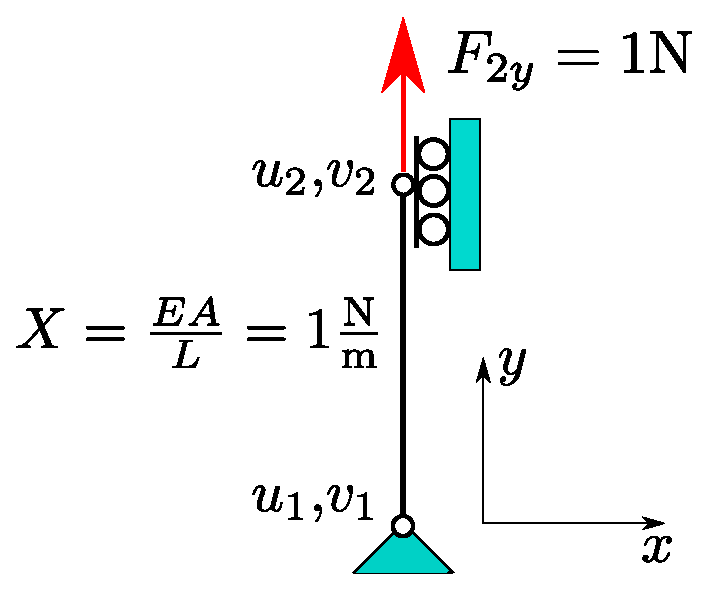
\includegraphics[width=0.4\textwidth]{fig/barpatch.eps}
	\caption{Un \textit{bar element test} para verificar un \textit{solver} de elementos finitos. $v_2=1$m.}
	\label{fig:barpatch}
\end{figure}

El \textit{bar element test} se puede mallar como un problema plano en el plano $xy$ con dos nodos ($x_1=y_1=x_2=0$, $y_2=1$m) y un elemento que los une. La rigidez del material entonces seria $EA=1$N. Se aplican las condiciones de borde detalladas en la figura: se restringen $u_1$,$v_1$ y $u_2$ y se resuelve el sistema para obtener $v_2$. Con este element test se verifica el método de resolución, la forma en que se rota la matriz de rigidez de la barra, la aplicación de condiciones de borde y el elemento en si. 


\section{Viga 3D de Timoshenko}
\begin{figure}[htb!]
	\centering
	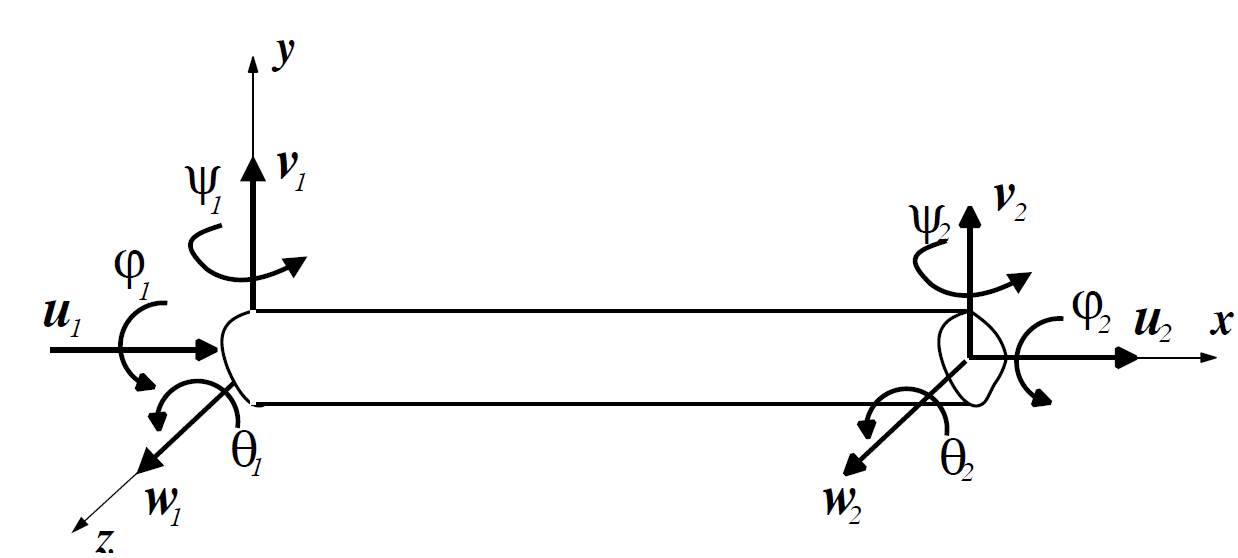
\includegraphics[width=0.6\textwidth]{fig/3dbeam.PNG}
	\caption{Grados de libertad (\textit{dof}) y coordenadas locales de una viga 3D de dos nodos y 6 dof por nodo.}
\end{figure}
La viga de Timoshenko 3D tiene las siguientes funciones de forma (forma eficiente tomada de \cite{luo2008efficient})
\[
\begin{cases}
\!\!\!\!\!
\begin{array}{l}
N_{1}=1-\xi \\
N_2 = \xi \\
\end{array}\Bigg\}\quad  \text{Funciones de forma para barras}\\
H_{v_{1}}=\beta_{y}\left(2 \xi^{3}-3 \xi^{2}+\alpha_{y} \xi+1-\alpha_{y}\right)\\
H_{v_{2}}=\beta_{y}\left(-2 \xi^{3}+3 \xi^{2}-\alpha_{y} \xi\right) \\
H_{w_{1}}=\beta_{z}\left(2 \xi^{3}-3 \xi^{2}+\alpha_{z} \xi+1-\alpha_{z}\right) \\
H_{w_{2}}=\beta_{z}\left(-2 \xi^{3}+3 \xi^{2}-\alpha_{z} \xi\right)\\
H_{\theta_{1}}=L \beta_{y}\left[\xi^{3}+\left(\frac{1}{2} \alpha_{y}-2\right) \xi^{2}+\left(1-\frac{1}{2} \alpha_{y}\right) \xi\right] \\
H_{\theta_{2}}=L \beta_{y}\left[\xi^{3}-\left(1+\frac{1}{2} \alpha_{y}\right) \xi^{2}+\left(\frac{1}{2} \alpha_{y}\right) \xi\right] \\
H_{\psi_{1}}=L \beta_{z}\left[\xi^{3}+\left(\frac{1}{2} \alpha_{z}-2\right) \xi^{2}+\left(1-\frac{1}{2} \alpha_{z}\right) \xi\right] \\
H_{\psi_{2}}=L \beta_{z}\left[\xi^{3}-\left(1+\frac{1}{2} \alpha_{z}\right) \xi^{2}+\left(\frac{1}{2} \alpha_{z}\right) \xi\right] \\
G_{v_{1}}=\frac{6 \beta_{y}}{L}\left(\xi^{2}-\xi\right) \\
G_{v_{2}}=\frac{6 \beta_{y}}{L}\left(-\xi^{2}+\xi\right) \\
G_{w_{1}}=\frac{6 \beta_{z}}{L}\left(\xi^{2}-\xi\right) \\
G_{w_{2}}=\frac{6 \beta_{z}}{L}\left(-\xi^{2}+\xi\right) \\
G_{\theta_{1}}=\beta_{y}\left[3 \xi^{2}+\left(\alpha_{y}-4\right) \xi+1-\alpha_{y}\right] \\
G_{\theta_{2}}=\beta_{y}\left[3 \xi^{2}-\left(\alpha_{y}+2\right) \xi\right] \\
G_{\psi_{1}}=\beta_{z}\left[3 \xi^{2}+\left(\alpha_{z}-4\right) \xi+1-\alpha_{z}\right] \\
G_{\psi_{2}}=\beta_{z}\left[3 \xi^{2}-\left(\alpha_{z}+2\right) \xi\right]
\end{cases}
\]
donde $x'$ es la coordenada local sobre la viga:
\[
\xi=\frac{x'}{L}, \qquad \alpha_{y}=\frac{12 E I_{y}}{k G A L^{2}}, \qquad \beta_{y}=\frac{1}{1-\alpha_{y}}, \qquad \alpha_{z}=\frac{12 E I_{z}}{k G A L^{2}},\qquad \beta_{z}=\frac{1}{1-\alpha_{z}}
\]
donde $k$ es el \textbf{factor de corrección por corte}\footnote{Ideado por Timoshenko en 1921 para permitir un mejor cálculo de las frecuencias naturales \cite{dong2010much}.} y depende de la sección y del modulo de Poisson $\nu$. Algunos valores en la tabla \ref{tab:kcorrectionfactor} del anexo.

Estas funciones de forma interpolan los desplazamientos sobre la viga:

\begin{equation} \label{eq:interpolacionFuncForma1D}
	\begin{cases}
	u=N_{1} u_{1}+N_{2} u_{2} \\
	v=H_{v_{1}} v_{1}+H_{\theta_{1}} \theta_{1}+H_{v_{2}} v_{2}+H_{\theta_{2}} \theta_{2} \\
	w=H_{w_{1}} w_{1}+H_{\psi_{1}} \psi_{1}+H_{w_{2}} w_{2}+H_{\psi_{2}} \psi_{2} \\
	\varphi=N_{1} \varphi_{1}+N_{2} \varphi_{2} \\
	\theta=G_{v_{1}} v_{1}+G_{\theta_{1}} \theta_{1}+G_{v_{2}} v_{2}+G_{\theta_{2}} \theta_{2} \\
	\psi=G_{w_{1}} w_{1}+G_{\psi_{1}} \psi_{1}+G_{w_{2}} w_{2}+G_{\psi_{2}} \psi_{2}
	\end{cases}
\end{equation} 



para luego calcular los esfuerzos usando las mismas formulas vistas en estática y resistencia de materiales.
\begin{align*}
	M_{z}&=E I_{z} \frac{\di^{2} v}{\di x^{2}}, \qquad V_{y}=\frac{\di M_{z}}{\di x}=E I_{z} \frac{\di^{3} v}{\di x^{3}}, \qquad N_x=A E \frac{u_{2}-u_{1}}{L} \\
	\qquad T&=G J_T \frac{\varphi_{2}-\varphi_{1}}{L}, \qquad M_{y}=E I_{y} \frac{\di^{2} w}{\di x^{2}}, \qquad V_{z}=E I_{y} \frac{\di^{3} w}{\di x^{3}}
\end{align*}
donde $J_T$ es la constante torsional de la viga y $A$ es la sección. \footnote{La constante torsional $J_T$ es igual a $I_p$ para secciones de viga circulares. Para perfiles abiertos de paredes delgadas, como por ejemplo un perfil doble T o un perfil `C', $J_T$ es mucho mas chico que $I_p$.}

La matriz de rigidez se puede obtener\footnote{Para una viga uniforme con sección simétrica y de  material en su rango elástico.} integrando analíticamente a la funciones de forma mencionadas anteriormente sobre el largo de la viga. En este documento no se va tratar la matriz de rigidez que resulta de dicha integración. Se presenta al lector la matriz de rigidez de una viga Timoshenko 3D clásica \cite{cook2007concepts}:

\begin{equation}\label{eq:matrizRigidezTimoshenko} \Mme{k'}_{\mathrm{1D}} = \left[\begin{array}{cccccccccccc} X & 0 & 0 & 0 & 0 & 0 & -X & 0 & 0 & 0 & 0 & 0\\ 0 & Y_{1} & 0 & 0 & 0 & Y_{2} & 0 & -Y_{1} & 0 & 0 & 0 & Y_{2}\\ 0 & 0 & Z_{1} & 0 & -Z_{2} & 0 & 0 & 0 & -Z_{1} & 0 & -Z_{2} & 0\\ 0 & 0 & 0 & S & 0 & 0 & 0 & 0 & 0 & -S & 0 & 0\\ 0 & 0 & -Z_{2} & 0 & Z_{3} & 0 & 0 & 0 & Z_{2} & 0 & Z_{4} & 0\\ 0 & Y_{2} & 0 & 0 & 0 & Y_{3} & 0 & -Y_{2} & 0 & 0 & 0 & Y_{4}\\ -X & 0 & 0 & 0 & 0 & 0 & X & 0 & 0 & 0 & 0 & 0\\ 0 & -Y_{1} & 0 & 0 & 0 & -Y_{2} & 0 & Y_{1} & 0 & 0 & 0 & -Y_{2}\\ 0 & 0 & -Z_{1} & 0 & Z_{2} & 0 & 0 & 0 & Z_{1} & 0 & Z_{2} & 0\\ 0 & 0 & 0 & -S & 0 & 0 & 0 & 0 & 0 & S & 0 & 0\\ 0 & 0 & -Z_{2} & 0 & Z_{4} & 0 & 0 & 0 & Z_{2} & 0 & Z_{3} & 0\\ 0 & Y_{2} & 0 & 0 & 0 & Y_{4} & 0 & -Y_{2} & 0 & 0 & 0 & Y_{3} \end{array}\right]\begin{array}{c}
u_1\\
v_1 \\
w_1 \\
\varphi_1 \\
\psi_1 \\
\theta_1 \\
u_2\\
v_2 \\
w_2 \\
\varphi_2 \\
\psi_2 \\
\theta_2 
\end{array}
\end{equation} 
donde  
\begin{align*}
	X&=\frac{AE}{L}, \qquad Y_4 = \frac{2EI_z}{L}, \qquad Y_3 = 2Y_4, \qquad Y_2 = \frac{3Y_4}{L} ,\qquad Y_1 = \frac{2Y_2}{L} \\
	Z_4 &= \frac{2EI_y}{L}, \qquad Z_3=2Z_4, \qquad Z_2 = \frac{2Z_4}{L}, \qquad Z_1 = \frac{2Z_2}{L}, \qquad S = \frac{G J_T}{L}
\end{align*}

\subsection*{Rótulas}

\begin{figure}[htb!]
	\centering
	\begin{subfigure}{0.49\textwidth}
		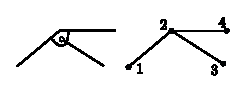
\includegraphics[width=\linewidth]{fig/rotulaexample.eps}
		\caption{Una unión rotulada y una posible discretización.}
		\label{fig:rotulaexample}
	\end{subfigure}
		\begin{subfigure}{0.49\textwidth}
	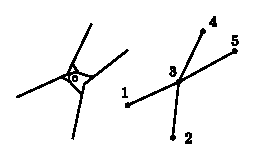
\includegraphics[width=\linewidth]{fig/rotulaexample2.eps}
	\caption{Dos sistemas de vigas unidos por una rótula y una posible discretización.}
	\label{fig:rotulaexample2}
	\end{subfigure}
    \caption{}
\end{figure}



Las uniones rotuladas permiten que ciertos elementos giren libremente manteniendo rigidez ante la rotación de otros elementos. El primer paso consiste en \textbf{desacoplar} el/los\footnote{Suponiendo que la figura \ref{fig:rotulaexample} está contenida en el plano $xy$: el giro a desacoplar sería en $z$ ($\theta$) dado la geometría de la rótula.} giro/s del elemento rotulado. Esto se logra generando un nuevo grado de libertad para cada giro desacoplado, el cual \textit{no pertenece a ningún nodo}, un \textit{nodeless dof}. Este nuevo dof se puede introducir al final de la matriz de rigidez para no estropear el mapeo de dof visto anteriormente. Al momento de acoplar la rigidez del elemento a la matriz de rigidez global la matriz \texttt{elemdof} (sección \ref{sec:dofmapping}) tiene que mostrar este cambio con los dof desacoplados. Para el caso de la figura \ref{fig:rotulaexample} con grados de libertad $u,v,\theta$ por nodo:

\begin{equation*} \label{eq:elemdofParaRotulaEjemplo}
\texttt{elementos} = \begin{bmatrix}
1 & 2  \\
2 & 4 \\
3 & 2\\
\end{bmatrix},
\qquad
\texttt{elemdof} = \begin{bmatrix}
1 & 2 & 3 & 4 & 5 & 6 \\
4 & 5 & 6 & 10 & 11 & 12  \\
7 & 8 & 9 & 4 & 5 & 13 \\
\end{bmatrix}
\end{equation*}
note que el elemento rotulado comparte los desplazamientos $u,v$ sobre el nodo 2 (dof 4 y 5) con los otros dos elementos pero tiene su giro $\theta$ desacoplado.

\textit{¿Como quedaría la matriz \texttt{elemdof} del sistema de la figura \ref{fig:rotulaexample2}?}


\section{Orientación de elementos 1D} \label{sec:OrientacionElementos}
Los elementos detallados en la sección anterior están acostados sobre el eje $x$. Para orientar un elemento en el espacio se tiene que empezar de hablar de una \textit{matriz de rotación} $\Mme{T}$.

\begin{equation} \label{eq:rotacionElemento}
	\Mk_{\mathrm{rotada}}= \Mme{T}^T \Mme{k'} \Mme{T}
\end{equation}
donde $\Mme{k'} $ es la matriz de rigidez local del elemento 1D antes de ser rotado. Luego de ser rotada la matriz puede ser acoplada a la rigidez global del sistema $\MK$.

Cabe agregar que los desplazamientos relacionados con el sistema global corresponden a los ejes globales. Para obtener los desplazamientos locales de los elementos se tienen que rotar estos también!

\begin{equation} \label{eq:rotacionDesplazamientos}
\Cme{d'}= \Mme{T} \Cme{d}  
\end{equation}
donde $\Cme{d'}$ son los desplazamientos del elemento en las coordenadas locales. Obtener $\Cme{d'}$ resulta útil al momento de querer calcular las fuerzas\footnote{El signo negativo es para obtener las fuerzas \textbf{internas} actuando en el elemento.} locales del elemento: \( \Mme{k'}\Cme{d'}= - \Cme{r'} \) o para interpolar los desplazamientos usando las expresiones en \eqref{eq:interpolacionFuncForma1D}.

\subsection*{Orientación de barras en el plano} \label{sec:OrientacionBarras}
La matriz de rigidez de una barra es definida horizontal. Esto significa que toda la rigidez está en $x$.

Una barra rotada $\phi$ grados va tener una nueva rigidez en el eje global $x$, e incluso puede no tener rigidez si se rota 90 grados.

La matriz transformación de una barra en el plano está dada por 

\[
\Mme{T}_{\mathrm{Barra}}= \begin{bmatrix}
\cos \phi & 0 \\
\sin \phi & 0 \\
0 & \cos \phi \\
0 & \sin \phi
\end{bmatrix}
\]

\subsection*{Orientación de vigas en el espacio}
Para orientar una viga se tiene que aportar más información que para una barra. Mientras que una barra se puede orientar con el simple input de sus nodos, la viga de Timoshenko necesita orientar su eje $y'$ además de su eje $x'$ .

Algunos programas como \Adina, por ejemplo, permiten al usuario especificar un nodo auxiliar o un vector auxiliar que apunta en la dirección en la cual se desea que la viga tenga su eje $y'$. 

Supongamos que elegimos este vector auxiliar $s_y=[0,1,0]$.\footnote{\textbf{Ser cauteloso al elegir el vector $s_y$ para que bajo ninguna circunstancia quede colineal al eje $x'$ del elemento. Esto causará problemas insanables.}} Esto nos va dar el mayor momento ante la flexión para una carga en $y$ global (suponiendo que $I_z>I_y$).
 \newcommand{\versor}[1]{\hat{#1}}
Para hallar la matriz de transformación $\Mme{T}$ debemos buscar los cosenos directores de nuestra viga en el espacio. Una vez que obtenemos el versor de orientación\footnote{Es el que resulta de la resta entre los nodos del elemento.} $\versor{v}_x$ es trivial obtener $\versor{v}_z$
\[
\versor{v}_z = \frac{\versor{v}_x\times s_y}{||\versor{v}_x\times s_y||}
\]
Luego de armar los versores $\versor{v}_x$, $\versor{v}_y$, $\versor{v}_z$ se define la matriz de los cosenos directores $\pmb{\lambda}$

\[
\pmb{\lambda} = \begin{bmatrix}
\versor{v}_x \\
\versor{v}_y \\
\versor{v}_z 
\end{bmatrix}_{3\times3}
\]

La matriz de transformación entonces es

\begin{equation}
	\Mme{T}_{\mathrm{1D}}=\begin{bmatrix}
	\pmb{\lambda} & &\cdots & 0 \\
	 &\pmb{\lambda} &  &\vdots \\
	\vdots & &\pmb{\lambda} & \\
	0 &\cdots & & \pmb{\lambda}
	\end{bmatrix}_{12\times 12}
\end{equation}
\input{\feaPP}

\section{Cargas}
\subsection*{Cargas Consistentes}
Una carga distribuida en $-y'$ sobre una viga que está fija en sus extremos tiene las cargas nodales

\begin{equation} \label{eq:CargaDistribuidaElemento}
	\Cme{r'} = \begin{Bmatrix}
	0 \\
	-qL/2 \\
	0\\
	0\\
	0\\
	-qL^2/12\\
	0\\
	-qL/2 \\
	0\\
	0\\
	0\\
	qL^2/12
	\end{Bmatrix}
	\qquad q \text{  en } \left[\frac{\text{Fuerza}}{\text{Longitud}} \right]
\end{equation}
estas son las cargas \textbf{\textit{consistentes}} porque toman en cuenta los momentos generados. Si se omiten los momentos se llaman \textit{cargas reducidas}.

Si la viga tiene una carga distribuida sobre su eje $y'$ local pero está arbitrariamente orientada se pueden obtener las cargas globales a aplicar sobre los nodos del elemento usando la matriz de rotación usada para orientar el elemento

\begin{equation}
	\Cme{r}= \Mme{T}^T \Cme{r'}
\end{equation}
usando $\Cme{r'}$ de \eqref{eq:CargaDistribuidaElemento}. Si la carga no está sobre el eje $y'$ de la viga, se deberá usar una matriz de rotación diferente, o cambiar el vector de cargas predefinido. \textit{¿Como aplicaría un par torsor a una viga arbitrariamente orientada?}
 \clearpage
\section{Ejercicios}
\subsection*{Pórticos}

\begin{figure}[htb!]
	\centering
	\begin{subfigure}{0.49\linewidth}
		\centering
		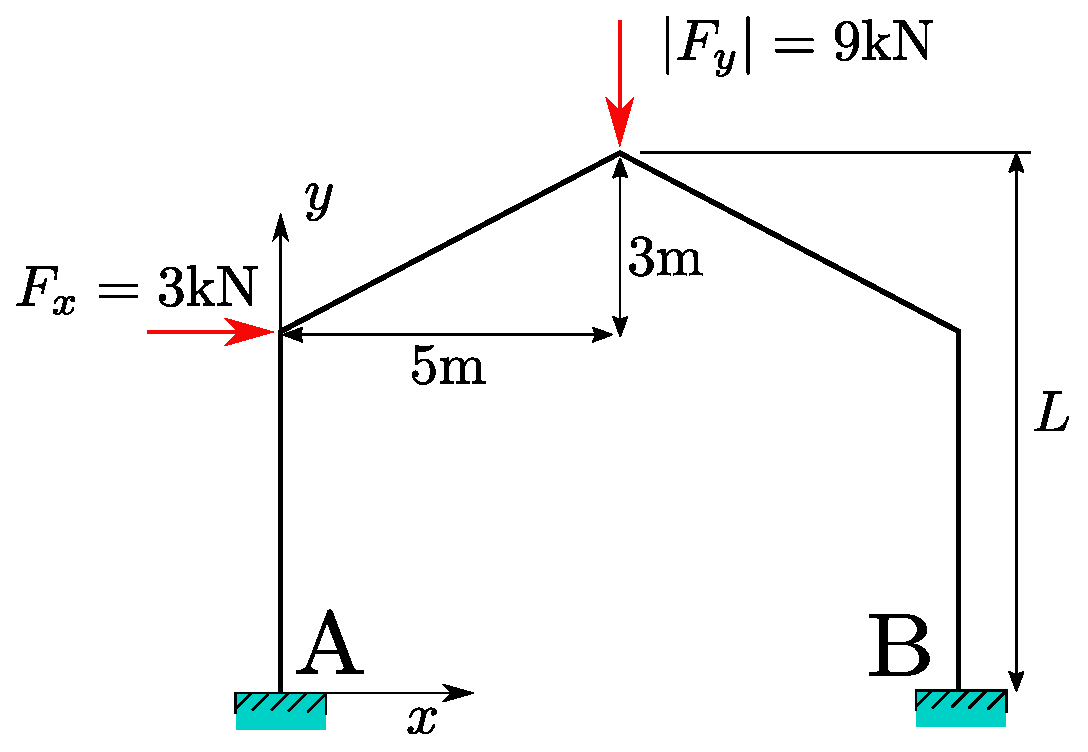
\includegraphics[width=1\textwidth]{fig/ej1viga.eps}
		\caption{Pórtico de altura $L$ a escala para el problema \ref{ej:probvigaaltura} }
		\label{fig:ej1viga}
	\end{subfigure}
	\begin{subfigure}{0.49\linewidth}
		\centering
	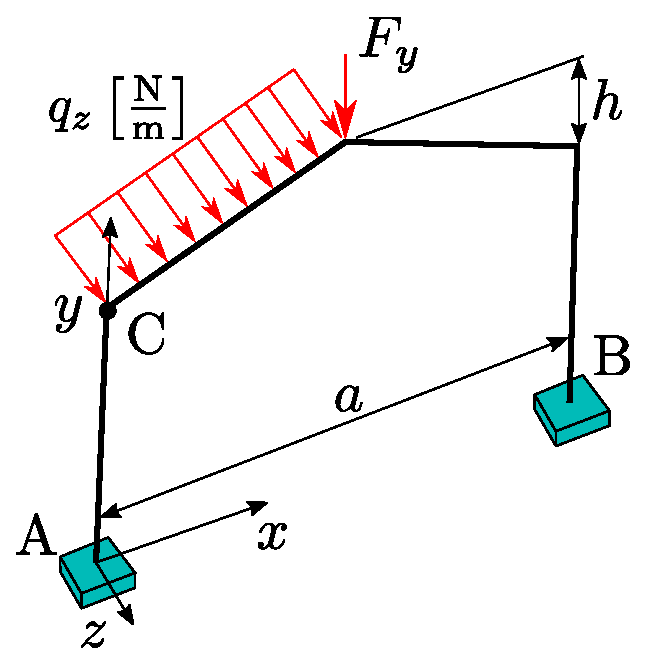
\includegraphics[width=.663\textwidth]{fig/ej2viga.eps}
	\caption{Pórtico con una carga distribuida en dirección $z$}
	\label{fig:ej2viga}
	\end{subfigure}
\caption{}
\label{fig:ejPorticos}
\end{figure}
\begin{enumerate}
	\item Para la figura \ref{fig:ej1viga} efectuar un modelo matemático y luego discretizar para resolver:
	\begin{enumerate}
		\item Verificar que para el caso dado con $F_x=0$ las reacciones en $y$ de los empotramientos son $\frac{F_y}{2}$.
		\item Se diseño el pórtico con una altura $L=7$ metros con perfiles IPN 160. Un análisis preliminar de una consultora sugiere que el punto superior supera los desplazamientos máximos permitidos de $d_{\max}=15$mm. Verificar.\label{ej:porticoVerificarConsultora}
		\item ¿Que altura debería el pórtico así el punto superior no se desplaza mas que $26.7$mm? Usar perfil IPB\footnote{Se puede buscar también como perfil HEB.} 120. ¿Es esta la configuración de la figura \ref{fig:ej1viga}? (\textit{hint:} si lo es)\label{ej:probvigaaltura}
	\end{enumerate}
	\item Para la figura \ref{fig:ej2viga} considerar perfiles HEB 340. 
	\begin{enumerate}
		\item Las reacciones considerando $a=12$m, $h=2$m  y una altura de $8$m. $q_z=500$ y $F_y=20$kN. \label{ej:reaccionportico3D}
		\item ¿Que orientación de vigas es favorable para reducir el desplazamiento del punto C?\label{ej:favorableportico3D} 
	\end{enumerate}
\end{enumerate}
Algunas Respuestas considerando $E=200$GPa:
\begin{itemize}
	\item[\ref{ej:porticoVerificarConsultora})]$d=0,0155$m, $\Cme{R_A}\approx\{1,1;\ms4,1;\ms-1,28\}$ kN o kNm
	
	\item[\ref{ej:reaccionportico3D})] $\Cme{R_B}\approx
	\{-6,2;\ms    10;\ms   -0,79;\ms   -0,64;\ms   -6,4;\ms   -0,5;\ms   16\}$ kN o kNm, con cargas reducidas
	
	\item[\ref{ej:favorableportico3D})] $d_{\mathrm{C}}=2,38$mm
	
\end{itemize}
\clearpage
\part{Elementos 2D}

%\section{Protips para el mallado}
Para mallar como un pro, empezar dividiendo el dominio. Cosas a tener en mente:
\begin{itemize}
	\item \textbf{Donde está la sección de mi dominio que quiero estudiar}? Puedo refinar en esa zona?
	\item Que orientación va tener mi malla para cada división de dominio?
	\item Que forma tendrán mis elementos con una dada división? Habrá una mejor forma de dividir mi dominio así no tengo jacobianos estramboticos?
\end{itemize}


\begin{figure}[htb!]
	\centering
	\begin{subfigure}{0.49\textwidth}
		\centering
		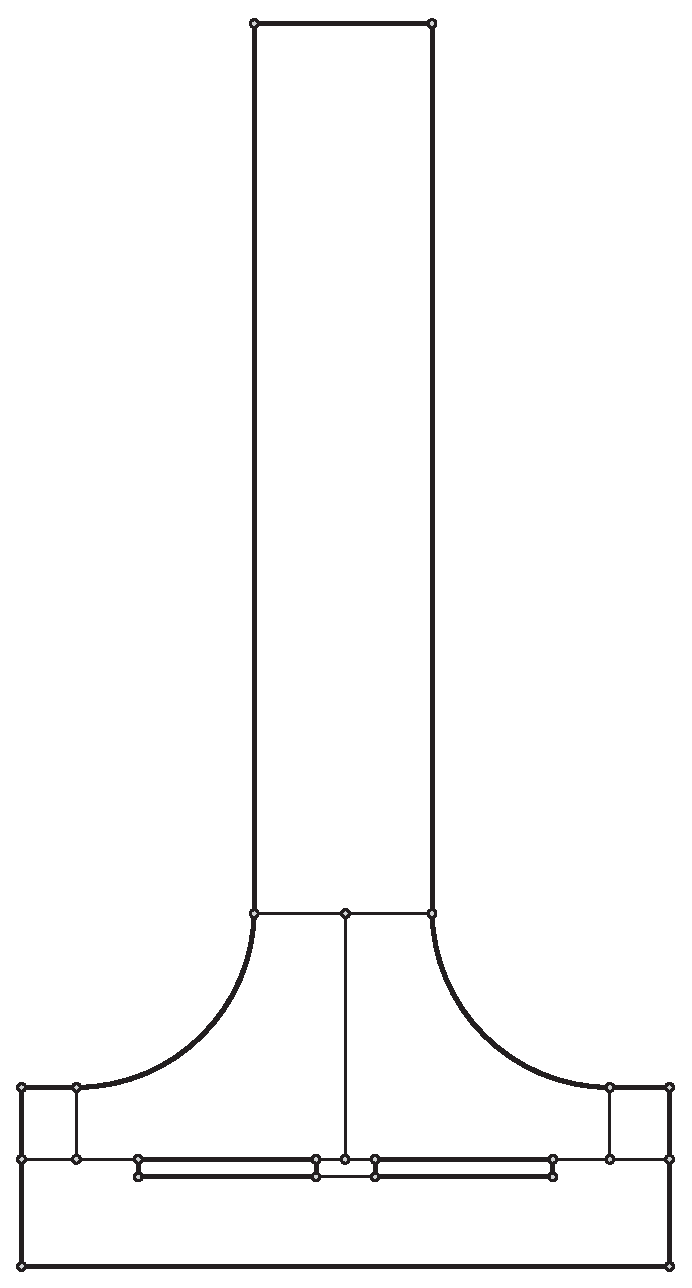
\includegraphics[width=.7\linewidth]{fig/divisionPelton1.eps}
		\caption{Mallable con triángulos solamente.}
	\end{subfigure}
	\begin{subfigure}{0.49\textwidth}
		\centering
	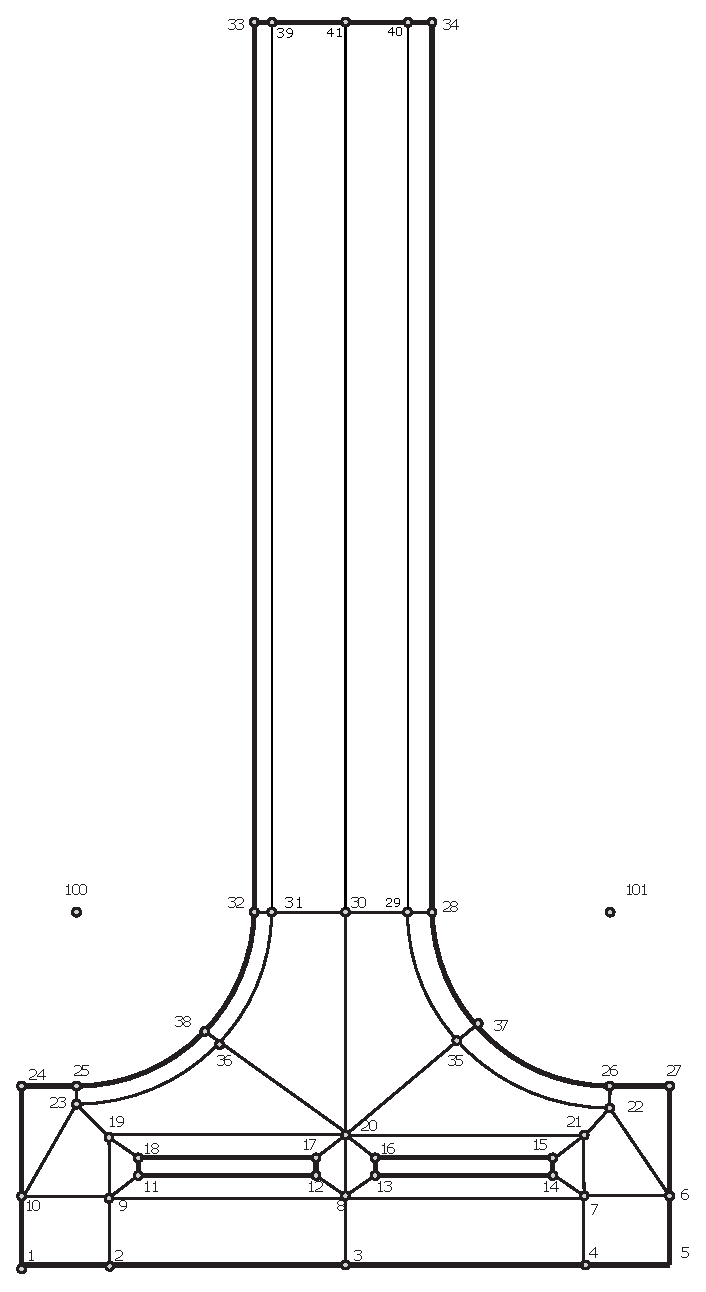
\includegraphics[width=.7\linewidth]{fig/divisionPelton2.eps}
	\caption{Se puede mallar con elementos cuadrilateros. No hay esquinas angulosas. Es posible obtener \textit{una buena malla}. Los nodos 100 y 101 son auxiliares y no forman parte de la malla.}
	\label{fig:buendivisiondominio}
	\end{subfigure}
	\caption{Dos formas de dividir una paleta de una turbina pelton que recibe un chorro incidente en su esquina superior derecha.}
\end{figure}
\begin{figure}[htb!]
	\centering
	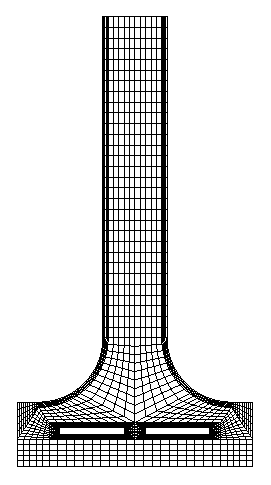
\includegraphics[angle=90,width=\linewidth]{fig/mallaPelton.eps}
	\caption{Ejemplo de malla usando divisiones de  \ref{fig:buendivisiondominio}. Se refina en los costados donde se tiene flexión.}
\end{figure}

%\clearpage
Protip: Necesitas saber que fuerza se tiene que hacer para que se mantenga en posición una arista o punto dado cargas térmicas/fuerza? Apoyalo (fix) y mira las reacciones con la carga térmica/fuerza.






\section{Funciones de formas para elementos 2D}
Se define cuantos nodos se va tener por elemento y se los ubica en el espacio $(\xi,\eta)$ que por simplicidad se trataran como $(x,y)$. Con el triangulo de Pascal para polinomios se elige el grado del polinomio y los términos. Luego se resuelve el sistema de ecuaciones $\MN\cdot X= A$ donde $\MN=[N_1\ms N_2 \ms \ldots\ms N_n]$ y $X=[1\ms x\ms y \ms\ldots\ms x^{k-1}y^{k} \ms x^{k}y^{k}]^T$, o algo por el estilo. Se tienen que elegir los grados mas convenientes teniendo en cuenta la simetría y el número de nodos, este ultimo te limita el número de términos posibles por la naturaleza de la interpolación. La matriz $A$ tendrá en su \textbf{espacio fila} el mismo polinomio evaluado en la posición del nodo correspondiente a esa fila.

\[
A=
\begin{bmatrix}
    1 & x_1 & y_1 & \dots  & x_{1}^{k-1}y_1^{k} & x_{1}^{k}y_1^{k} \\
    1 & x_2 & y_2 & \dots  & x_{2}^{k-1}y_2^{k} & x_{2}^{k}y_2^{k} \\
    \vdots & \vdots & \vdots & \ddots & \vdots& \vdots \\
    1 & x_n & y_n & \dots  & x_{n}^{k-1}y_n^{k} & x_{n}^{k}y_n^{k}
\end{bmatrix}
\]
Luego, las funciones de forma $\MN$ se pueden obtener así: $\MN=X^{-1} A$

\section*{Cargas 2-D}
La ecuación que rige como se cargan elementos, siendo $\Cme{r}$ las cargas nodales del elemento, $\Cme{F}$ fuerzas volumétricas, $\CPhi$ fuerzas de tracción superficiales, $\Cme{\varepsilonb_0}$ las deformaciones iniciales y $\Cme{\sigmab_0}$ las tensiones iniciales (pg. 228)
\begin{equation} \label{eq:CargasGenerales}
\Cme{r}=\overbrace{\int \MN^T \Cme{F} \di V}^{\text{Volumétricas}} + \overbrace{\int \MN^T \CPhi \di S}^{\text{Superficiales}}+\int \MB^T \ME \Cme{\varepsilonb_0} \di V- \int \MB \Cme{\sigmab_0} \di V
\end{equation}



\section{Elementos isoparamétricos}
\begin{itemize}
    \item Un elemento que no esta distorsionado (sigue siendo rectangular) tiene $J$ constante
    \item Cuidado con modo espurio. Ver tabla 6.8-1 pg. 226 el tema de full/reduced integration \cite{cook2007concepts}
    \item Como cargar tu elemento isoparamétrico en pg. 228
\end{itemize}

\begin{figure}[htb!]
    \centering
    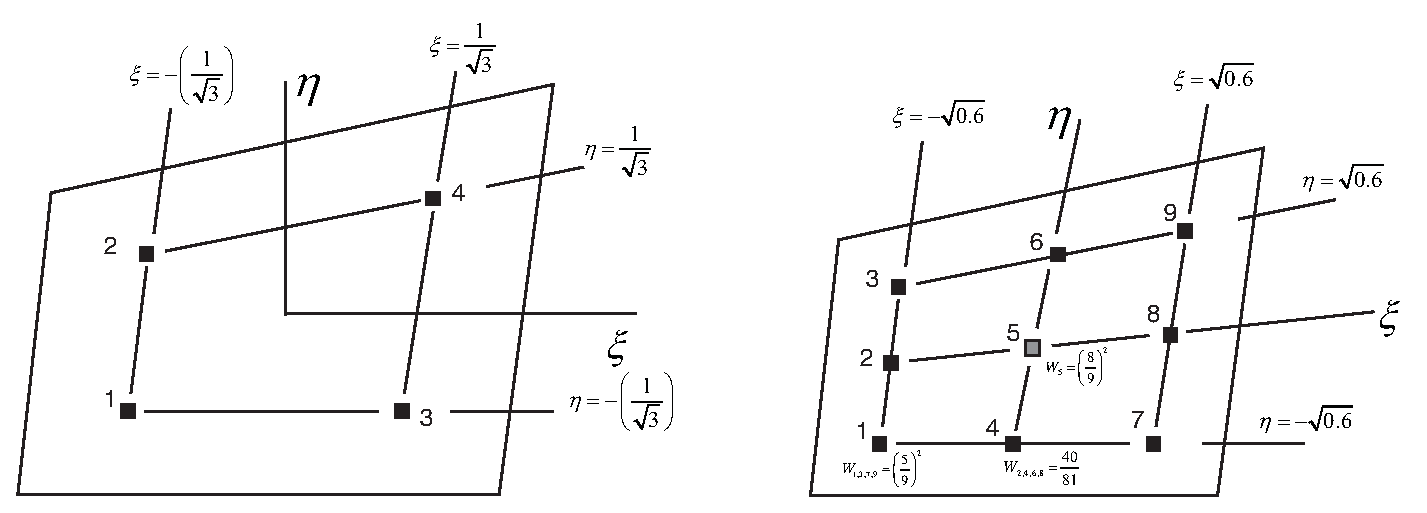
\includegraphics[width=12cm]{fig/gauss_n3.eps}
    \caption{Puntos gauss para ordenes $n=2$ y $n=3$. El peso para $n=2$ es igual en todos los puntos $W_i=1$}
    \label{fig:gauss_n3}
\end{figure}

\section*{Ejemplo elemento exótico}
\subsection*{Matriz de Rigidez}
Imaginemos un elementos Q5 cuadrado de $2\times2$ con espesor $t$  (igual al Q4 con un nodo en su centro). Si fuéramos a obtener las funciones de formas de dicho elemento quedarían iguales para $(x,y)$ y para $(\xi,\eta)$ por las dimensiones usadas. La funcionalidad que uno estaría tentado a seleccionar sería $[1,\ x, \ y,\ x^2, \ y^2 ]$, pero está trae problemas inesperados debido a que tiene varias soluciones en la interpolación. Como nuestra prioridad siempre es mantener la simetría la funcionalidad será $[1,\ x,\ y,\ xy,\ x^2y^2 ]$.  Tomando el orden de la figura \ref{fig:elemq5}.
\[
\MN=\left[\begin{array}{ccccc} \frac{x^2\,y^2}{4}+\frac{x\,y}{4}-\frac{x}{4}-\frac{y}{4}, & \frac{x^2\,y^2}{4}-\frac{x\,y}{4}+\frac{x}{4}-\frac{y}{4}, & \frac{x^2\,y^2}{4}+\frac{x\,y}{4}+\frac{x}{4}+\frac{y}{4}, & \frac{x^2\,y^2}{4}-\frac{x\,y}{4}-\frac{x}{4}+\frac{y}{4}, & 1-x^2\,y^2 \end{array}\right]
\]

Llegado a este punto nos interesa obtener la matriz de rigidez. Si queremos lograr \emph{``full integration"} deberíamos usar Gauss orden $n=3$ según $2n-1\geq O\left(\MB^T \ME \MB \right)$. $\MB$ es el \textit{strain-deformation matrix}. El producto $\MB^T \ME \MB$ da un polinomio de orden 6 ($\MB$ tiene el mismo orden que la derivada de $\MN$). De esta forma nos aseguramos que nuestro resultado va ser exacto para el elemento sin distorsionar.

Para esté ejemplo, no se pide \emph{full integration} entonces no pasa nada si queremos \emph{underintegrate}. Usamos Gauss orden $n=2$. 

\begin{figure}[htb!]
    \centering
    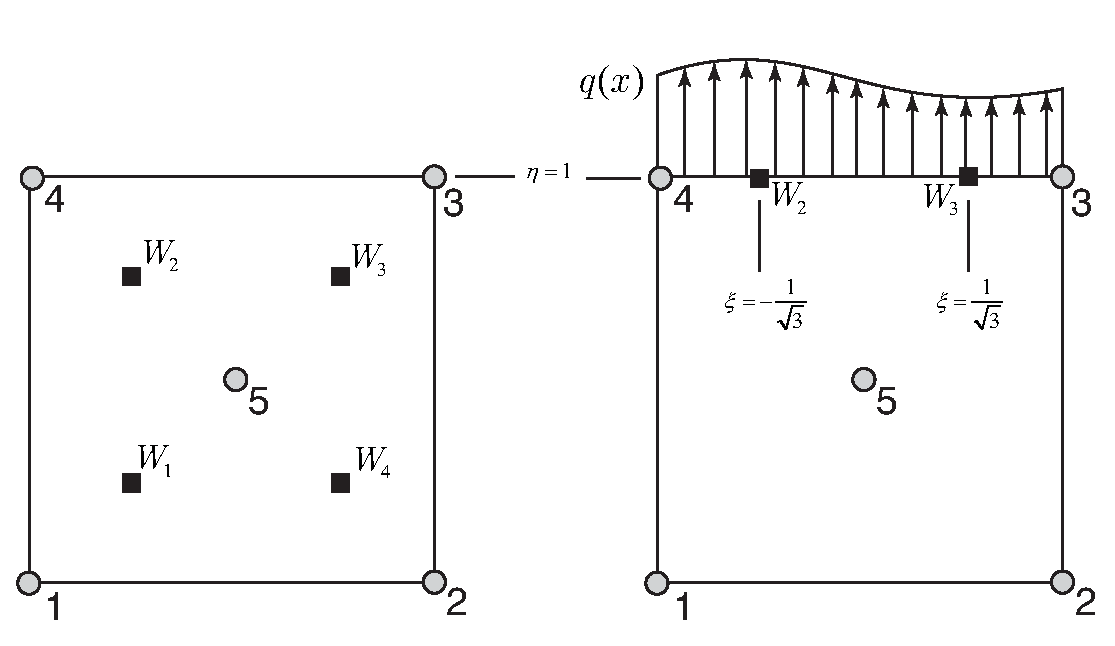
\includegraphics[height=5cm]{fig/exoticElement.eps}
    \caption{Elemento Q5 rectangular.}
    \label{fig:elemq5}
\end{figure}

La rigidez de un elemento está dada por 


\begin{equation} \label{eq:RigidezElemento}
    \Mk=\int \MB^T \ME \MB \di V
\end{equation}
para un elemento plano la ecuación anterior es
\[
\Mk_{\mathrm{2D}}=\iint \MB^T \ME \MB t \di x \di y=\int^1_{-1}\int^1_{-1} \MB^T \ME \MB t \ \Djac \  \di\xi  \di\eta
\]
donde $\MB$ es la matriz deformación-desplazamiento del elemento, $\ME$ es la matriz constitutiva, y $\Djac$ es el determinante de la matriz Jacobiana, el cual se le suele decir simplemente el Jacobiano.

Este ultimo se calcula a partir de la derivada de las funciones de forma $ $

\subsection*{Carga de linea}
 Si el elemento está cargado sobre la linea 4-3 con una distribuida $q(x)$ (en [\si{\newton \per \meter}]) entonces procedemos de la siguiente manera según el segundo término de \refp{eq:CargasGenerales}: 

\begin{align}
r_{xi}&=\int^1_{-1}N_i (\tau \jac_{11}- \sigma \jac_{12})t\di \xi \\
r_{yi}&=\int^1_{-1}N_i (\sigma \jac_{11}+\tau \jac_{12})t \di \xi 
\end{align}
donde $\sigma$ es la solicitación normal a la superficie y $\tau$ es la tangencial. Para la fuerza sobre el nodo 4 se tiene

$$r_{y4}= N_4(\xi_2)t\left[\sigma(\xi_2)\; \jac_{11}+\tau(\xi_2)\; \jac_{12}\right] \cdot W_2 + N_4(\xi_3)t\left[\sigma(\xi_3)\; \jac_{11}+\tau(\xi_3)\; \jac_{12}\right]\cdot W_3 $$

Si consideramos que solo hay una \emph{carga distribuida de linea} a tracción/compresión como indica la figura \ref{fig:elemq5}, se reduce la ecuación anterior

$$ r_{y4} = N_4(\xi_2)\;\jac_{11}\;q(\xi_2) + N_4(\xi_3)\;\jac_{11}\;q(\xi_3) =N_4\;q \;\jac_{11}\Big|_{\xi_2} + N_4\;q\; \jac_{11}\Big|_{\xi_3} $$
similarmente $r_{y3} = N_3\;q \;\jac_{11}\big|_{\xi_2} + N_3\;q\; \jac_{11}\big|_{\xi_3} $ donde la matriz Jacobiana también se evalúa para cada punto de Gauss!


\subsection*{Tensiones}
    \begin{itemize}
        \item Las tensiones en los nodos suele ser de mayor interés que sobre los puntos de gauss (mas comprometidas, permiten estimar error)
    \end{itemize}

 \input{\feaSP}
\section{Elementos Axisimetricos}
Resuelvo problema 3-D en el plano. Los resultados son por cada unidad radian. Como sigo teniendo dos grados de libertad tengo las mismas funciones de forma. Cambia mi operador derivada.
\[
\begin{Bmatrix}
    \sigma_\radial \\
    \sigma_\theta \\
    \sigma_z \\
    \tau_{z\radial}
\end{Bmatrix}
= \frac{(1-\nu)E}{(1+\nu)(1-2\nu)}
\begin{bmatrix}
   1 & \eff & \eff & 0 \\
    & 1 & \eff & 0 \\
    & & 1 & 0 \\
    \textrm{sim.}\unspace& & & g 
\end{bmatrix}
\left(
\begin{Bmatrix}
\varepsilon_\radial \\
\varepsilon_\theta \\
\varepsilon_z \\
\gamma_{\radial z}
\end{Bmatrix}
-
\begin{Bmatrix}
\alpha T\\
\alpha T \\
\alpha T \\
0
\end{Bmatrix}
\right)
\]
donde 
\[
f=\frac{\nu}{1-\nu}\qquad \quad \textrm{y}\quad \qquad g=\frac{1-2\nu}{2(1-\nu)}
\]

Una carga puntual $P$ aplicada sobre un elemento axisimétrico no tiene el mismo significado físico que en elementos plane stress/strain. 
\[
P=2\pi rq
\]
donde $q$ es la carga distribuida en [N/m], $r$ es la distancia al eje de revolución y $2 \pi$ es el resultado de integrar la fuerza distribuida sobre $\theta$. 

\[
\Cme{r_e} = \int\int_{-\pi}^{\pi} \MN^T \begin{Bmatrix}
    \rho r \omega ^2 \\
    0
\end{Bmatrix} r \di \theta \di A
\]
\part{Otras cosas}

\section{Desplazamientos iniciales} \label{sec:desplzImpuestos}
Si nuestro sistema tiene desplazamientos iniciales conocidos se puede formular un sistema a resolver:

\begin{equation}
	\begin{bmatrix}
	\MKxx & \MKxc \\
	\MKcx & \MKcc
	\end{bmatrix}
	\begin{Bmatrix}
	\CDx \\
	\CDc 
	\end{Bmatrix}
	=	\begin{Bmatrix}
	\CRc \\
	\CRx 
	\end{Bmatrix}
\end{equation} 
Note que para los nodos donde se conocen los desplazamientos (los nodos $\mathrm{c}$) \textit{se desconocen las cargas}, por ende las cargas sobre los nodos con desplazamientos conocidos tienen subíndice $\mathrm{x}$. La rigidez del sistema $\MK{}$ es conocida; se usan los subindices $\mathrm{x}$ y $\mathrm{c}$ solo para tener referencia. El sistema expandido tiene la forma
\begin{gather*} 
	\MKxx \CDx + \MKxc \CDc = \CRc \\
	\MKcx \CDx + \MKcc \CDc = \CRx 
\end{gather*}
La matriz $\MKxx$ no es singular si se impusieron suficientes desplazamientos como para prevenir movimiento de cuerpo rígido/mecanismos. Se pueden entonces obtener los desplazamientos desconocidos
\[
\CDx = \MKxx^{-1} \left( \CRc - \MKxc  \CDc \right)
\]
luego de obtener los desplazamientos desconocidas se puede obtener las cargas desconocidas $\CRx$.

\input{\feaTP}

\section{Restricciones}
Las restricciones sirven para imponer una nueva relación a los dof del sistema ya existente $Kd=F$. Las condiciones de borde esenciales son restricciones de un punto. Se pueden tener restricciones \textit{multi punto} al relacionar los dof entre si como es el caso para rigid links.

\subsection*{Multiplicadores de Lagrange}

\begin{equation}
	\begin{bmatrix}
	\mathbf{K} & \mathbf{C}^T\\
	\mathbf{C} & 0
	\end{bmatrix}
	\begin{Bmatrix}
	\mathbf{D} \\
	\pmb{\lambda}
	\end{Bmatrix}
	=
	\begin{Bmatrix}
	\mathbf{R} \\
	\mathbf{Q}
	\end{Bmatrix}
\end{equation}
El sistema de desconocidas se vuelve los desplazamientos $\CD$ y un vector de multiplicadores de Lagrange $\pmb{\lambda} $. $\mathbf{Q}$ es el lado derecho de la ecuación de restricciones. La ventaja de este método es su resultado exacto.

\subsection*{Método del penal}
\begin{equation}
	(\mathbf{K}+\alpha \mathbf{C}^T \mathbf{C})\mathbf{D} = \mathbf{R} + \alpha \mathbf{C}^T \mathbf{Q}
\end{equation}
$\alpha$ es una constante de magnitud relativamente grande en comparación al máximo de la diagonal de $\mathbf{K}$. Lo que se hace es agregar un valor alto a matriz de rigidez y una fuerza correspondiente para cumplir la restricción. 

La gran ventaja de este método es que se conserva el tamaño del sistema a resolver resultando en tiempos de resolución cortos para sistemas con muchas restricciones. Las desventajas también son importantes tomar en cuenta: Para un resultado más exacto es necesario agrandar $\alpha$. El usuario también tiene que tener cuidado que si se aumenta un $\alpha$ que multiplica un elemento no-diagonal entonces pueden llegar a haber problemas numéricos de acondicionamiento. 

\subsection*{Armado de $\mathbf{C}$}
Si se quiere restringir dos dof con una relación del tipo $u_n=u_m$ entonces la ecuación es
\[
\Mme{c}^T_{\Ndof \times 1} = \begin{bmatrix}
0 \\ 
\vdots \\
1 \\
\vdots \\
-1 \\
\vdots \\
0
\end{bmatrix}\begin{array}{c}
u_1\\
\vdots \\
u_m \\
\vdots \\
u_s \\
\vdots \\
u_{\Nnod}
\end{array}
,
\qquad 
\mathbf{q} = 0
\qquad \Rightarrow \quad u_m-u_s = \mathbf{q} = 0
\]
donde el nodo $m$ es el \textbf{master} y el nodo $s$ es el \textbf{slave}. Cuando se tengan varias restricciones unidas a un nodo, este nodo será el \textbf{master} y se tendrán que plantear las ecuaciones adecuadamente para que sea así.

 Algunas reglas generales para guiarse con elementos rígidos:
\begin{enumerate}
	\item Un nodo slave restringido tiene solo un master para que hay a una solución definida
	\item Un nodo no puede ser slave y master a la vez
\end{enumerate}


\subsection*{Rigid Bar en el plano}
Un rigid bar o un rigid beam (son restricciones inherentemente distintas) cumple la función de unir dos nodos con un elemento 1D totalmente rígido. Aunque se podría hacer con un elemento barra con rigidez alterada artificialmente, esto puede traer problemas numéricos si la rigidez alterada es muy alta. Además, para el estudio de dinámica estructural y vibraciones es indeseable tener elementos con rigidez artificialmente alta pues agregan modos de alta frecuencia. Estos modos después hacen que el análisis dinámico transitorio sea imposible de efectuar. Para estos casos se emplean los multiplicadores de Lagrange.

\begin{figure}[htb!]
	\centering
	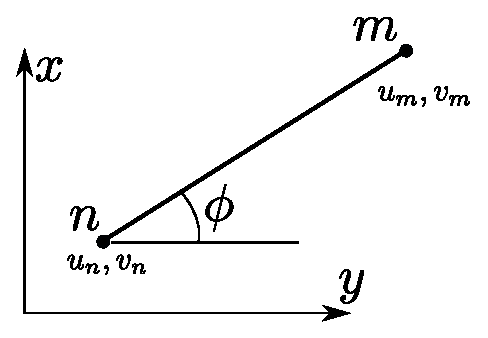
\includegraphics[width=7cm]{fig/rigidbarschematic.eps}
	\caption{Un rigid bar que une el nodo $n$ con el nodo $m$.}
	\label{fig:rigidbarschematic}
\end{figure}

El motivo del rigid bar es un elemento que \textit{no se acorta ni se alarga} con las fuerzas que transmite. Un usuario del método de elementos finitos podría pensar que alcanza con plantear dos ecuaciones $u_n=u_m$;$v_n=v_m$ sin embargo esto lograría que los nodos $n$ y $m$ se trasladen como un cuerpo rígido sin permitir rotaciones, efectivamente logrando una rigidez más alta que la propuesta en el motivo del rigid bar.

Si el rigid bar de la figura \ref{fig:rigidbarschematic} permite rotaciones sin acortarse, entonces la distancia que se mueve el nodo $m$ sobre el eje local $x'$ del rigid bar debe ser igual al del nodo $n$, dando una única ecuación
\[
u_n\cos\phi + v_n \sin\phi = u_m\cos\phi +v_m\sin\phi  
\]
esta restricción se puede agregar al sistema usando los multiplicadores de Lagrange o con el método del penal.


\subsection*{Rigid beam en el plano}
En el análisis ingenieril por FEA es común el uso de restricciones para modelar roscas, unir elementos con dof disimiles, etcætera. Para el segundo caso se puede usar un \textit{rigid link} (rigid beam) para transmitir rotaciones de un elemento/nodo con giro a un elemento sin giros en sus nodos, como podría ser el caso de unión viga-elemento 3D.

La formulación de un rigid link consiste en plantear ecuaciones de cinemática para una viga rígida (considerando desplazamientos pequeños). Los desplazamientos cartesianos del nodo slave serán condicionados por los giros del nodo master

\begin{align*}
	u_s &= u_m  + L_e \versor{v}_y\theta_m \\
	v_s &= v_m  - L_e \versor{v}_x \theta_m \\
	\theta_s &= \theta_m
\end{align*}
donde $L_e$ es la distancia entre nodo slave y master.

La formulación para un rigid link en el espacio puede ser deducida de la formulación RBE2 en el anexo de este documento planteando desplazamientos pequeños.

\section{Error}

Para calcular error ZZ primero se obtiene un campo de tensiones que ``mejor aproxima la solucion''{} llamado el \textbf{smoothed field} o campo suavizado ($\sigma^*$). Hay varios metodos para obtener $\sigma^*$, en este documento se va tratar el método de suavizado por elemento.

\subsection*{Element smoothing}
Se obtienen las tensiones sobre los puntos gauss superconvergentes mediante la ecuacion
\[
 \Cme{\sigmab^*}_i = \Mme{E} \Mme{B^*} \Cme{d}
\]
donde $\Mme{B^*}$ es obtenida integrando sobre dichos puntos de gauss. Esto nos da el campo suavizado $\sigma^*$ del elemento. 

\subsection*{Error ZZ}
Para poder integrar las siguientes expresiones se tendrá que obtener $\Cme{\sigmab}_i$ sobre los puntos de cuadratura, es decir, habrá que interpolar el campo no-suavizado sobre los puntos gauss. En general no son idénticas las dos tensiones. Recordar que no tiene sentido obtener $\eta$ sobre un dominio que presenta discontinuidades de tensiones inherentes, como cambios abruptos de sección y cambio de material.
\[
\vvert{U}^2 = \sum^m_{i=1}\int_{v_e} \Cme{\varepsilonb}_i^T \ME \Cme{\varepsilonb}_i \di V
\]
donde $m$ es el numero de elementos del dominio donde se quiere calcular $\eta$.
\[
\vvert{e}^2=\sum_{i=1}^m \int_{v_e} \left( \Cme{\varepsilonb^*}_i - \Cme{\varepsilonb}_i\right)^T \ME \left( \Cme{\varepsilonb^*}_i - \Cme{\varepsilonb}_i\right) \di V
\]

\[
\vvert{e}^2=\sum_{i=1}^m \int_{v_e} \left( \Cme{\sigmab^*}_i - \Cme{\sigmab}_i\right)^T \ME ^{-1} \left( \Cme{\sigmab^*}_i - \Cme{\sigmab}_i\right) \di V
\]

El error relativo ($\eta$) esta comprendido entre 1 y 0. Un valor aceptable de $\eta$ suele ser tomado como $\eta\leq 0,05$ \citep{cook2007concepts}.
\[
\eta = \sqrt{\frac{\vvert{e}^2}{\vvert{e}^2+\vvert{U}^2}}
\]


\section{Transferencia de Calor}

Tenemos el flujo de calor que es $\underline{K} \nabla T$, la divergencia de esto es el flujo neto que pasa por un punto.
\[
\nabla(\underline{K} \nabla T)+Q=\rho c \frac{\partial T}{\partial \tau}
\] 

Ley de Newton: 
\[
q_{c}=h_{c}(s, T)\left(T-T_{\infty}\right)
\]

Ley de Stefan Boltzmann
\[
q_{r}=\varepsilon_{r} \sigma\left(T^{4}-T_{\infty}^{4}\right)
\]

Es mas complicado el tema de modelar temperaturas fijas e imponer calor transferido, pues son aseveraciones no tan reales como imponer desplazamiento cero sobre un apoyo y  fuerzas sobre vigas.

Para aplicar convección 

Hay una parte que depende de la temperatura interna, la parte que no depende la dejo como vector de cargas. La parte que depende la tengo que sumar a mi matriz de conductividades
\[
R_{C_{i}}=\oint_{\Gamma_{c o m v}} N_{i} h\left(T(x)-T_{f l}\right) d \gamma
\]

Lo escribe sebas: $kT=q_c = HT-RT_{fl} \longrightarrow (K-H)T = -R T_{fl}$

\[
\mathrm{Cargas:} R_{H} : \oint_{\Gamma_{c o n v}} N_{i} h T_{f l} d \gamma \qquad \qquad \mathrm{Conductividad:}  K : \oint_{\Gamma_{c m}} N_{i} h N_{j} d \gamma
\]


\subsection*{Resolución de problemas típico}

Condiciones de borde de temperatura. Idéntico a lo visto en la sección \ref{sec:desplzImpuestos}.

\[
\Cme{T_{\mathrm{x}}} = \Mme{K_{\mathrm{xx}}}^{-1} \left( \Cme{Q_\mathrm{x}}- \Mme{K_{\mathrm{xc}}}  \Cme{T_\mathrm{c}} \right)
\]
luego de obtener las temperaturas desconocidas se puede obtener el flujo desconocido (sobre los nodos conocidos):
\[
\Cme{Q_{\mathrm{c}}} = \Mme{K_{\mathrm{cx}}} \Cme{T_\mathrm{x}} + \Mme{K_{\mathrm{cc}}} \Cme{T_\mathrm{c}}  
\]





\section{Formulación elemento Hexaedro de 8 nodos}
\newcommand{\dof}{\ensuremath{\mathrm{dof}}}
El modelado con elementos isoparamétricos hexaedros de 8 nodos es un buen punto de partida para comenzar a manejar los elementos finitos en 3 dimensiones. Un código hecho para obtener $\MK$ con elementos H8 se adapta con facilidad para los H20.

\begin{figure}[htb!]
	\centering
	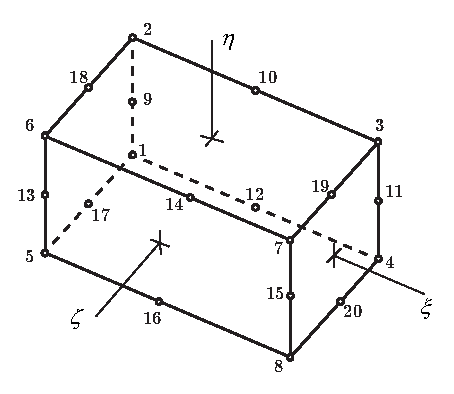
\includegraphics[width=.6\textwidth]{fig/H20numbering.eps}
	\caption{Numeración de nodos H20 en \Adina (Ejes sugeridos)}
	\label{fig:H20numbering}
\end{figure}

Cada nodo tendrá $3$ grados de libertad, dándonos $24$ \dof{} por elemento. El elemento H20 de la figura \ref{fig:H20numbering} esta planteado de tal forma que los primeros nodos del 1 al 8 son los nodos del H8 que se va formular a continuación.

La funcionalidad a usar es la siguiente

\[
X_{\mathrm{H8}} = \left[1, \xi, \eta, \zeta, \xi \eta, \xi \eta, \eta \zeta, \xi \eta \zeta \right]
\]


y la matriz constitutiva para sólidos 3D con 3 \dof{} por nodo se escribe:

\begin{equation}
	\ME =\left[\begin{array}{cccccc} 2\,G+\lambda  & \lambda  & \lambda  & 0 & 0 & 0\\ \lambda  & 2\,G+\lambda  & \lambda  & 0 & 0 & 0\\ \lambda  & \lambda  & 2\,G+\lambda  & 0 & 0 & 0\\ 0 & 0 & 0 & G & 0 & 0\\ 0 & 0 & 0 & 0 & G & 0\\ 0 & 0 & 0 & 0 & 0 & G \end{array}\right] \qquad \ME^{-1}=\frac{1}{E}\left[\begin{array}{cccccc} 1 & -\nu  & -\nu  & 0 & 0 & 0\\ -\nu  & 1 & -\nu  & 0 & 0 & 0\\ -\nu  & -\nu  & 1 & 0 & 0 & 0\\ 0 & 0 & 0 & f & 0 & 0\\ 0 & 0 & 0 & 0 & f & 0\\ 0 & 0 & 0 & 0 & 0 & f \end{array}\right]
\end{equation}
donde $\lambda = \frac{E \nu}{(1+\nu)(1-2\nu)}$ y $G=\frac{E}{2(1+\nu)}$ y $f = 2+2\nu$.

\subsubsection*{Formulación elementos}
El jacobiano tiene la forma
\[
\jac=
\left[\begin{array}{lll}\spartial{x}{\xi} & \spartial{y}{\xi}  & \spartial{z}{\xi}  \\ \spartial{x}{\eta}  &\spartial{y}{\eta}  &\spartial{z}{\eta} \\\spartial{x}{\zeta} & \spartial{y}{\zeta} &\spartial{z}{\zeta}\end{array}\right]
\]
pudiendo ser calculado de la siguiente forma

\begin{equation}
	\jac = \begin{bmatrix}
	\frac{\partial}{\partial \xi} \MN \\
	\frac{\partial}{\partial \eta} \MN \\
	\frac{\partial}{\partial \zeta} \MN 
	\end{bmatrix}
	\cdot 
\left[\begin{array}{lll}{x_{1}} & {y_{1}} & {z_{1}} \\ {x_{2}} & {y_{2}} & {z_{2}} \\ {x_{3}} & {y_{3}} & {z_{3}} \\ {x_{4}} & {y_{4}} & {z_{4}} \\ {x_{5}} & {y_{5}} & {z_{5}} \\ {x_{6}} & {y_{6}} & {z_{6}} \\ {x_{7}} & {y_{7}} & {z_{7}} \\ {x_{8}} & {y_{8}} & {z_{8}}\end{array}\right]
\end{equation}
donde la primer matriz termina siendo $3\times8$ para un elemento H8. La segunda matriz son las posiciones \textit{globales} de los nodos del elemento. El jacobiano se puede entonces utilizar para calcular

\begin{equation}
	\Mme{\partial N}=\left[\begin{array}{l} \frac{\partial}{\partial x}\MN  \\ \frac{\partial}{\partial y} \MN  \\ \frac{\partial}{\partial z} \MN  \end{array}\right]=\jac^{-1}\left[\begin{array}{l}\frac{\partial}{\partial \xi} \MN \\
	\frac{\partial}{\partial \eta} \MN \\ 
	\frac{\partial}{\partial \zeta} \MN \end{array}\right]
\end{equation}
con lo obtenido se puede calcular la matriz $\MB$.

La matriz \textit{strain-deformation} queda
\[
\MB = \begin{bmatrix}
B_1 &B_2 &B_3 &B_4 &B_5 &B_6 &B_7 &B_8
\end{bmatrix}
\]
donde
\begin{equation}
B_{i}=\left[\begin{array}{ccc}{\partial N_{i} / \partial x} & {0} & {0} \\ {0} & {\partial N_{i} / \partial y} & {0} \\ {0} & {0} & {\partial N_{i} / \partial z} \\ {0} & {\partial N_{i} / \partial z} & {\partial N_{i} / \partial y} \\ {\partial N_{i} / \partial z} & {0} & {\partial N_{i} / \partial x} \\ {\partial N_{i} / \partial y} & {\partial N_{i} / \partial x} & {0}\end{array}\right]
\end{equation}

Finalmente un calcula la rigidez del elemento usando \eqref{eq:RigidezElemento}.






\part{No-linealidad y análisis dinámico}

\section{Respuesta dinámica estructural}

\begin{equation} \label{eq:ecuacionDinamicaGeneral}
	\Mme{M}\Cme{\boldsymbol{\ddot{\mathrm{D}}}} + \Mme{C}\Cme{\boldsymbol{\dot{\mathrm{D}}}}+\Mme{K} \Cme{D} =\Cme{R^{\mathrm{ext}}}
\end{equation}

Se puede resolver la ecuación de arriba para un sistema dado sin amortiguamiento y sin cargas externas\footnote{Se denomina vibración ``libre'' cuando no hay cargas asociadas. Si no hay amortiguamiento el desplazamiento es regido por $u= \bar{u}\sin \omega t$, donde $\bar{u}$ es la amplitud de vibración y $\omega$ es la frecuencia circular \cite{cook2007concepts}. $\omega$ es obtenida en radianes por segundo.} para obtener sus frecuencias naturales y los modos asociados a estos.
\[
\CD = \Cme{\boldsymbol{\bar{\mathrm D}}}\sin \omega t, \qquad \Cme{\boldsymbol{\ddot{\mathrm{D}}}}= -\omega^2 \Cme{\boldsymbol{\bar{\mathrm D}}} \sin \omega t
\]
sin considerar la matriz de amortiguamiento se obtiene el problema de autovalores:

\[
\left( \MK - \omega^2 \Mme{M} \right)\Cme{\boldsymbol{\bar{\mathrm D}}} = \Cme{0}
\]
donde $\omega^2$ es un autovalor y la raíz de estos son las frecuencias naturales.




Amortiguamiento $\Mme{C} = \alpha \Mme{M}+\beta \Mme{K}$ cede una matriz no diagonal. Se complica la resolución. Existen dos otros modelos que tratan con una matriz $\Mme{C\modal}$ diagonal donde las ecuaciones se desacoplan.


Amortiguamiento Modal: Se elige un $\dampfact$ para cada modo
\begin{equation}
\Mme{C\modal}=\left[ \begin{array}{ccc}{2 \omega_{n} \dampfact_{n}} & {0} & {0} \\ {0} & {\ddots} & {0} \\ {0} & {0} & {2 \omega_{1} \dampfact_{1}}\end{array}\right]
\end{equation}

Amortiguamiento proporcional. Se basa el análisis 

\begin{equation}
	\Mme{C\modal} = \Mme{\Phib}^T ( \alpha \Mme{M}+\beta \Mme{K})\Mme{\Phib} = \alpha \delta \Mme{I} +\beta \Mme{\Omegab^2}
\end{equation}

Si se quiere estudiar un rango de frecuencias de excitación tal que $\omega_{\mathrm{exc}}\in [\omega_1, \omega_2]$ y eligiendo dos valores de damping para ambas frecuencias $\dampfact_1$ y $\dampfact_2$ se tiene:
\begin{align*}
\alpha &= 2\omega_1 \omega_2 (\dampfact_1 \omega_2 -\dampfact_2 \omega_1)/(\omega_2^2 - \omega_1^2) \\ \beta &= 2(\dampfact_2\omega_2 -\dampfact_1 \omega_1)/(\omega_2^2 - \omega_1^2)
\end{align*}

Una vez obtenida $\Mme{C\modal}$ se pueden obtener los desplazamientos modales $\Cme{Z}$. Tome en cuenta que debido a la diagonalidad de $\Mme{\Omegab^2}$ y $\Cme{R\modal }$ se desacoplan las ecuaciones de \ref{eq:ecuacionDinamicaGeneral} y por ende se pasa a tratar dichas matrices diagonales como vectores columnas. Una vez desacopladas se tiene
 \[\Cme{\boldsymbol{\ddot{\mathrm{Z}}}}+2\COmega \Cme{C\modal} \Cme{\boldsymbol{\dot{\mathrm{Z}}}} + \Cme{\Omegab^2} \Cme{Z} = \Cme{R\modal} \]
\[
\Cme{Z} = \frac{\Cme{R\modal }}{ \Cme{\Omegab^2} \sqrt{(1-\chi^2)^2 + (2 \Cme{C\modal} \chi)^2}}
\]
donde $\chi = \frac{\omega_{\mathrm{exc}}}{\COmega}$. 



\subsection*{Sine Sweep}
A medida que la frecuencia de excitación aumenta la \textit{amplitud del sistema disminuye}\footnote{Excepto en cercanías de una frecuencia natural}. Es interesante pensar que si aumentara no tendría sentido buscar las frecuencias naturales porque estas son caracterizadas por un máximo de amplitud. Las curvas del barrido de frecuencia son decrecientes en lejanía de una frecuencia natural porque para una fuerza cíclica $F(t)=F_0\sin \omega t$ el tiempo que actúa en una dirección es inversamente proporcional a la frecuencia. Por ende la estructura no tiene tiempo para moverse lejos antes de que se invierta la dirección de la fuerza.

\subsection*{Matriz de masa consistente para una viga 3D}
  \begin{equation}
  	\Mme{m}_{\mathrm{1D}} = \int_0^L \MN^T \MN \rho A \di x
  \end{equation}
  La matriz de masa según una fuente desconocida
  \begin{equation}
  	\Mme{m'}_{\mathrm{1D}}= \frac{\rho A L}{420}\left[\begin{array}{cccccccccccc} 140 & 0 & 0 & 0 & 0 & 0 & 35 & 0 & 0 & 0 & 0 & 0\\ 0 & 156 & 0 & 0 & 0 & 22\,L & 0 & 27 & 0 & 0 & 0 & -13\,L\\ 0 & 0 & 156 & 0 & -22\,L & 0 & 0 & 0 & 27 & 0 & 13\,L & 0\\ 0 & 0 & 0 & 140\,{r_{x}}^2 & 0 & 0 & 0 & 0 & 0 & -35\,{r_{x}}^2 & 0 & 0\\ 0 & 0 & -22\,L & 0 & 16\,L^2 & 0 & 0 & 0 & -13\,L & 0 & -6\,L^2 & 0\\ 0 & 22\,L & 0 & 0 & 0 & 16\,L^2 & 0 & 13\,L & 0 & 0 & 0 & -6\,L^2\\ 35 & 0 & 0 & 0 & 0 & 0 & 140 & 0 & 0 & 0 & 0 & 0\\ 0 & 27 & 0 & 0 & 0 & 13\,L & 0 & 156 & 0 & 0 & 0 & -22\,L\\ 0 & 0 & 27 & 0 & -13\,L & 0 & 0 & 0 & 156 & 0 & 22\,L & 0\\ 0 & 0 & 0 & -35\,{r_{x}}^2 & 0 & 0 & 0 & 0 & 0 & 140\,{r_{x}}^2 & 0 & 0\\ 0 & 0 & 13\,L & 0 & -6\,L^2 & 0 & 0 & 0 & 22\,L & 0 & 16\,L^2 & 0\\ 0 & -13\,L & 0 & 0 & 0 & -6\,L^2 & 0 & -22\,L & 0 & 0 & 0 & 16\,L^2 \end{array}\right]	
  \end{equation}
donde $r_x =\sqrt{ \frac{I_z}{A}}$. 


La matriz de masa según un paper escrito por \cite{matas2014study}
\[ \pmb{m_{11}}=
\left[\begin{array}{cccccc}{\frac{1}{3}} & {0} & {0} & {0} & {0} & {0} \\ {0} & {\frac{13}{35}} & {0} & {0} & {0} & {\frac{11 L}{210}} \\ {0} & {0} & {\frac{13}{35}} & {0} & {\frac{-11 L}{210}} & {0} \\ {0} & {0} & {0} & {\frac{I_{y}+I_{z}}{3 A}} & {0} & {0} \\ {0} & {0} & {\frac{-11 L}{210}} & {0} & {\frac{L^{2}}{105}} & {0} \\ {0} & {\frac{11 L}{210}} & {0} & {0} & {0} & {\frac{L^{2}}{105}}\end{array}\right], \quad \pmb{m_{12}}= \left[\begin{array}{cccccc}{\frac{1}{6}} & {0} & {0} & {0} & {0} & {0} \\ {0} & {\frac{9}{70}} & {0} & {0} & {0} & {\frac{-13 L}{420}} \\ {0} & {0} & {\frac{9}{70}} & {0} & {\frac{-13 L}{420}} & {0} \\ {0} & {0} & {0} & {\frac{I_{y}+I_{z}}{6 A}} & {0} & {0} \\ {0} & {0} & {\frac{-13 L}{420}} & {0} & {\frac{-L^{2}}{140}} & {0} \\ {0} & {\frac{13 L}{420}} & {0} & {0} & {0} & {\frac{-L^{2}}{140}}\end{array}\right]
\]

\[
\pmb{m_{21}} = \left[\begin{array}{cccccc}{\frac{1}{6}} & {0} & {0} & {0} & {0} & {0} \\ {0} & {\frac{9}{70}} & {0} & {0} & {0} & {\frac{13 L}{420}} \\ {0} & {0} & {\frac{9}{70}} & {0} & {\frac{-13 L}{420}} & {0} \\ {0} & {0} & {0} & {\frac{I_{y}+I_{z}}{6 A}} & {0} & {0} \\ {0} & {0} & {\frac{13 L}{420}} & {0} & {\frac{-L^{2}}{140}} & {0} \\ {0} & {\frac{-13 L}{420}} & {0} & {0} & {0} & {\frac{-L^{2}}{140}}\end{array}\right], \quad \pmb{m_{22}} = \left[\begin{array}{cccccc}{\frac{1}{3}} & {0} & {0} & {0} & {0} & {0} \\ {0} & {\frac{13}{35}} & {0} & {0} & {0} & {\frac{-11 L}{210}} \\ {0} & {0} & {\frac{13}{35}} & {0} & {\frac{11 L}{210}} & {0} \\ {0} & {0} & {0} & {\frac{I_{y}+I_{z}}{3 A}} & {0} & {0} \\ {0} & {0} & {\frac{11 L}{210}} & {0} & {\frac{L^{2}}{105}} & {0} \\ {0} & {\frac{-11 L}{210}} & {0} & {0} & {0} & {\frac{L^{2}}{105}}\end{array}\right]
\]
donde
\begin{equation}
	\Mme{m'}_{\mathrm{1D}}= \rho A L \left[\begin{array}{cc}
	\pmb{m_{11}}  &  \pmb{m_{12}} \\
	\pmb{m_{21}}  &  \pmb{m_{22}} 
	\end{array}\right]
\end{equation}
\section{Transferencia de calor no-lineal y transitoria}

\subsection*{Radiacion}
Cuando se tienen problemas de radiación se puede iterar para obtener el perfil usando \textbf{relajación.}


\begin{equation}
\begin{cases}
\CTx^{n+1}_{\mathrm{unrelaxed}} =  \MKxx^{-1}  \left(\CRx^{n} - \MKxc \CTc^{n}\right)\\
\CR^{n} = \Cme{R_{\mathrm{generado}}}+ \Cme{R_{\mathrm{rad}}}^{n} \\
\Cme{T}^{n+1} = \Cme{T}^n + \frac{1}{k_R} \cdot \left( \Cme{T}^{n+1}_{\mathrm{unrelaxed}} - \Cme{T}^{n} \right)
\end{cases}
\end{equation}
donde $k_R$ es la relajación o factor de atenuación de temperaturas. Cuanto mayor es más ``amortiguada'' es la convergencia del perfil. Usando mayores $k_R$ se puede asegurar la convergencia de la solución a costo de ser más lenta.


\subsection*{Transitorio}
Matriz capacidad
\[
[C]=\int_{\Omega}[N]^{T} \rho c[N] d \omega
\]
Temperature-Heat flux matrix $\MB$ para Q4:
\[
\MB =
\begin{Bmatrix}
\frac{\partial N}{\partial \xi} \frac{\partial \xi}{\partial x} + \frac{\partial N}{\partial \eta} \frac{\partial \eta}{\partial x} \\
\frac{\partial N}{\partial \xi} \frac{\partial \xi}{\partial y} + \frac{\partial N}{\partial \eta} \frac{\partial \eta}{\partial y} 
\end{Bmatrix}
\]

Si a beta le digo que vale cero el futuro muere en cambio si beta vale 1 entonces TODO depende del futuro.
\[
\beta[C]\{\dot{T}\}^{n+1}+(1-\beta)[C]\{\dot{T}\}^{n}+[K] \beta\{T\}^{n+1}+[K](1-\beta)\{T\}^{n}=(1-\beta)\left\{R_{T}\right\}^{n}+\beta\left\{R_{T}\right\}^{n+1}
\]

Ecuación iterativa:
\begin{equation}
\Cme{T}^{n+1} = \left( \MC +\Delta t \beta \MK \right)^{-1} \left[ \left(\MC -\Delta t(1-\beta) \MK\right) \Cme{T}^n +\Delta t \left( (1-\beta) \Cme{R}^n + \beta \Cme{R}^{n+1}  \right)\right]
\end{equation}



\[
\begin{array}{|l|l|}\hline \beta=0 & {\text {Euler Forward Difference }} \\ \hline \beta=0.5 & {\text {Crank--Nicholson }} \\ \hline \beta=0.666 & {\text {Galerkin }} \\ \hline \beta=1 & {\text {Backward Difference }} \\ \hline\end{array}
\]

\section{Análisis Dinámico}

\subsection*{Método Integración Directa}
Resuelve \ref{eq:ecuacionDinamicaGeneral}.
\begin{align*}
	\begin{cases}
	\Cme{V}^{n+1}&=\Cme{V}^n + \frac{\Delta t}{2}  \Mme{M}^{-1}\left(\Cme{R^{\mathrm{ext}}} - \MC \Cme{V} - \MK \Cme{D} \right) \\
	\Cme{D}^{n+1}&=\Cme{D}^n + \frac{\Delta t}{2} \Cme{V}
	\end{cases}
\end{align*}


\subsection*{Método Runge--Kutta K4}
Tengo que resolver las dos ecuaciones simultáneamente
\[
\begin{cases}
	\Cme{V}^{n+1}=\Cme{V}^n + \frac{\Delta t}{6} \left( \kuV + 2\kdV + 2\ktV + \kcV \right) \\
	\Cme{D}^{n+1}=\Cme{D}^n + \frac{\Delta t}{6} \left( \kuD + 2\kdD + 2\ktD + \kcD \right) \\
\end{cases}
\]
donde 
\begin{align*}
	\begin{cases}
	\kuV &= \Mme{M}^{-1} \left( \Cme{R^{\mathrm{ext}}}^n - \MC \Cme{V}^n - \MK \Cme{D}^n  \right) \\
	\kuD &= \Cme{V}^n \\\hline
	\kdV &= \Mme{M}^{-1} \left( \Cme{R^{\mathrm{ext}}}^{n+\frac{1}{2}} - \MC \left(\Cme{V}^n + \frac{\Delta t}{2} \kuV \right) - \MK \left( \Cme{D}^n + \frac{\Delta t}{2} \kuD \right)  \right) \\
	\kdD &= \Cme{V}^n + \frac{\Delta t}{2} \kuV \\	\hline
	\ktV &= \Mme{M}^{-1} \left( \Cme{R^{\mathrm{ext}}}^{n+\frac{1}{2}} - \MC \left(\Cme{V}^n + \frac{\Delta t}{2} \kdV \right) - \MK \left( \Cme{D}^n + \frac{\Delta t}{2} \kdD \right)  \right) \\
	\ktD &= \Cme{V}^n + \frac{\Delta t}{2} \kdV \\	\hline
	\kcV &= \Mme{M}^{-1} \left( \Cme{R^{\mathrm{ext}}}^{n+1} - \MC \left(\Cme{V}^n + \Delta t \ktV \right) - \MK \left( \Cme{D}^n + \Delta t \ktD \right)  \right) \\
	\kcD &= \Cme{V}^n + \Delta t \ktV
	\end{cases}
\end{align*}

\part{Métodos avanzados para la programación}
Esta sección incluye técnicas para facilitar la programación de modelos complejos (OOP) y estructuras de datos que optimizan el tiempo de corrida.

\section{OOP}
La programación orientada a los objetos (Objected Oriented Programming) tiene sus ventajas al momento de tratar programas complejos. \Matlab{} tiene una implementada una estructura de datos llamada \verb|struct| cuyo comportamiento es similar al de otros lenguajes OOP. 

Si se piensa que una variable es un cajón donde se puede guardar una matriz o string, un struct seria un mueble con amplio espacio para varios cajones. Los cajones se llaman \verb|fields| o campos. Crear un struct es tan fácil como agregar un punto entre dos nombres de variables:

\begin{lstlisting}[caption={Ejemplos de structs y como acceder a sus campos.}]
mueble.cajon1 = [0 1 2];  % mi struct se llama mueble
mueble.c2 = {'Ke','Ep','k'}; % cajon1 y c2 son campos del struct 
fprintf( '%d %s',mueble.cajon1(2),mueble.c2{1} )
\end{lstlisting}

Las ventajas solo resultan aparente cuando se tiene un código largo donde se tienen muchas variables. Su aplicación en los elementos finitos son numerosas, pues no presentan desventaja en el tiempo de corrida y suelen disminuir la complejidad del código.

\begin{itemize}
	\item Mas facilidad para funciones que llaman a structs. Resulta mas fácil modificar estas dado un cambio en el código
	\item Usar una struct para cada tipo o grupo de elemento para almacenar su matriz de rigidez, matriz elementos etc. reduce la complejidad del código
	\item Guardar resultados de una corrida es tan fácil como \verb|save('solucion.mat','structSolucion')| donde \verb|structSolucion| puede contener los desplazamientos, tensiones, reacciones etc.
\end{itemize}



\section{Integración pre-cargada}
No es necesario calcular las funciones de forma sobre los puntos gauss o nodos cada vez que se itera sobre un elemento, se pueden guardar estas en un cell array y llamarlas en el momento. El uso de este método puede reducir por un factor mayor a 10 el tiempo de corrida. A continuación se declara una estructura \verb|gp| que contiene toda la información relacionada a los puntos gauss, incluyendo

\begin{itemize}
	\item \verb|gp.n| La cantidad de puntos gauss a integrar
	\item \verb|gp.w| Los pesos de los puntos gauss
	\item \verb|gp.u| Las posiciones de los puntos gauss
	\item \verb|gp.N| Las funciones de forma de los nodos evaluadas en los puntos gauss (un cell array)
\end{itemize}

\subsubsection*{Creación del cell array}
\begin{lstlisting}[caption = {Creación de struct relacionada a los puntos de Gauss.}]
gp.N=cell(gp.n,1);
gp.dN= cell(gp.n,1);
for ipg =1:gp.n %Optimiza para problemas grandes 
   xi = gp.u(ipg,1); eta = gp.u(ipg,2);
   gp.N{ipg} = N(xi, eta);
   gp.dN{ipg} = dN(xi, eta);% funciones de formas derivadas
end
\end{lstlisting}

\subsubsection*{Integración pre-cargada}

\begin{lstlisting}[caption = {Aplicación del método de integración pre-cargada.}]
DOF = reshape(1:dof,Ndofpornod,[])';
for e = 1:Nelem
    ke = zeros(Ndofporelem);
    meindof = reshape(DOF(elementos(e,:),:)',1,[]);
    elenod = nodos(elementos(e,:),:);
    for ipg = 1:gp.n
        jac = gp.dN{ipg}*elenod; % estas dos lineas corren
        dNxyz = jac\gp.dN{ipg}; %mucho mas rapido que integracion lenta
        Djac = det(jac);
        B = zeros(size(E,2),Ndofporelem);
        %% Calculo B para mi elemento
        ke = ke + B'*E*B*gp.w(ipg)*Djac;
    end
    %Acople a matriz de rigidez K
end
\end{lstlisting}

\section{Acople rápido de \(\MK \)}

Se puede optimizar mucho el espacio en memoria cambiando la forma de almacenamiento de \(\MK \) a esparsa. Lo que no se sabe es que importa mucho la forma en que se acoplan los valores a \(\MK \). A continuación hay un esquema para el armado rápido de \(\MK \).

\subsubsection*{Declaración de indices y vector valor}
\begin{lstlisting}
I = zeros( Ndofporelem*Nelem ,1 ); %indice i de K
J = zeros( Ndofporelem*Nelem ,1 ); %indice j de K
V = zeros( Ndofporelem*Nelem ,1 ); %Valores de K
Nentryporelem = Ndofporelem^2; %Cantidad de valores en ke
n2de = @(e) repmat(Nentryporelem*e ,Nentryporelem ,1 ) - (Nentryporelem-1:-1:0)';
\end{lstlisting}

\subsubsection*{Acople Rápido}
\begin{lstlisting}[caption = {Aplicación del método de acople rápido de la matriz de rigidez.}]
for e = 1:Ndofporelem
    ke = zeros(Ndofporelem,Ndofporelem);
    meindof = reshape(DOF(elementos(e,:),:)',1,[]);
    elenod = nodos(elementos(e,:),:);
    % obtengo ke de alguna forma
    idx = n2de(e);
    I(idx) = repmat(meindof,1,Ndofporelem)' ;
    J(idx) = reshape(repmat(meindof,Ndofporelem,1),[],1);
    V(idx) = ke(:);
end

K = sparse( I, J, V , dof, dof); %spalloc rapido
\end{lstlisting}

Este método funciona muy bien para problemas con cientos de miles de dof. Para un problema de 600000 dof con elementos tetraedros de diez nodos (T10), este método permite pasar de un acople de 15.600 segundos (con integración rápida) a tan solo 50 segundos.

\section{Verificación de \(\MK \)}
\subsection*{Autovalores de $\MK$}
Tomando los autovalores de $\MK$ nos puede dar una buena idea de si nos falta aplicar condiciones de borde o si hay mal condicionamiento numérico. El problema de este método es que deja de funcionar para modelos con muchos dof ya que el calculo de autovalores es muy intensivo sobre los recursos de la computadora.
\begin{lstlisting}
    [autoval, autovec] =eigs(K(isfree,isfree));
\end{lstlisting}

La existencia de autovalores nulos o muy cercanos a cero puede implicar 
\begin{itemize}
    \item Existencia de modos rígidos de desplazamiento
    \item Una razón alta entre valores de la diagonal de $\MK$ y los no-diagonales (mal condicionamiento numérico)
\end{itemize}
\subsection*{Mecanismos y singularidades en NASTRAN}
Una vez armada la matriz de rigidez global resulta útil poder encontrar dofs que actúen como mecanismos o problemas de condicionamiento. Para esto NASTRAN implementa un método para hallar estos dofs. Primero se restringe \(\MK \) aplicando condiciones de borde esenciales y ecuaciones de restricciones. Luego se divide cada elemento de su diagonal ($\MK_{ii}$) por su elemento correspondiente de la matriz $D$ de la descomposición LDL, obteniéndose así los \textit{pivot-ratios}.

\[
\text{PIVOTRATIO} = \frac{\MK_{ii}}{D_{ii}}
\]

en \Matlab{} se puede vectorizar el problema
\begin{lstlisting}[caption = {Rutina MAXPIVOT de NASTRAN.}]
KLL = K(isfree, isfree); %Condiciones de borde
pivots = decomposition(KLL,'ldl','lower')\diag(KLL);
\end{lstlisting}
son de interés los dof con pivot ratio mas alto. NASTRAN pone un limite superior de $10^8$ antes de finalizar la corrida con un error.

Tenga cuidado al buscar el dof que causa el problema, pues redujo el problema aplicando condiciones de borde esenciales! 



\part{Anexo}

\section{Solver genérico para elementos 2D (Q4)} \label{sec:q4codigo}

\begin{figure}[ht!]
    \centering
    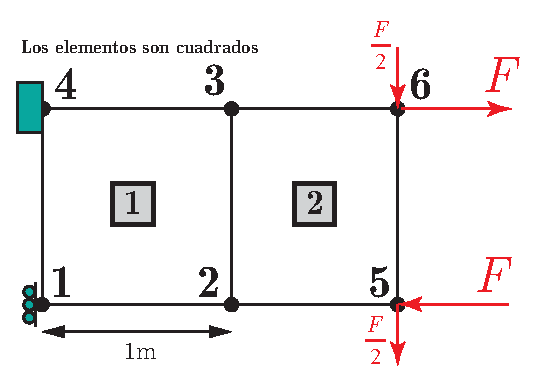
\includegraphics[width=0.5\textwidth]{fig/q4domain.eps}
    \caption{Problema plane-stress a resolver. $F=10$kN, $t=1$cm.}
\end{figure}

\lstinputlisting[caption = {q4shapefun.m}]{code/q4shapefun.m}
\lstinputlisting[caption = {q4solve.m}]{code/q4solve.m}
\lstinputlisting[caption = {q4stress.m}]{code/q4stress.m}
\lstinputlisting[caption = {q4graphstress.m}]{code/q4graphstress.m}
%set(gcf,'renderer','Painters');filename='q4domain';
%print('-depsc','-tiff','-r300', '-painters',[filename,'.eps'])
\begin{figure}[ht!]
    \centering
    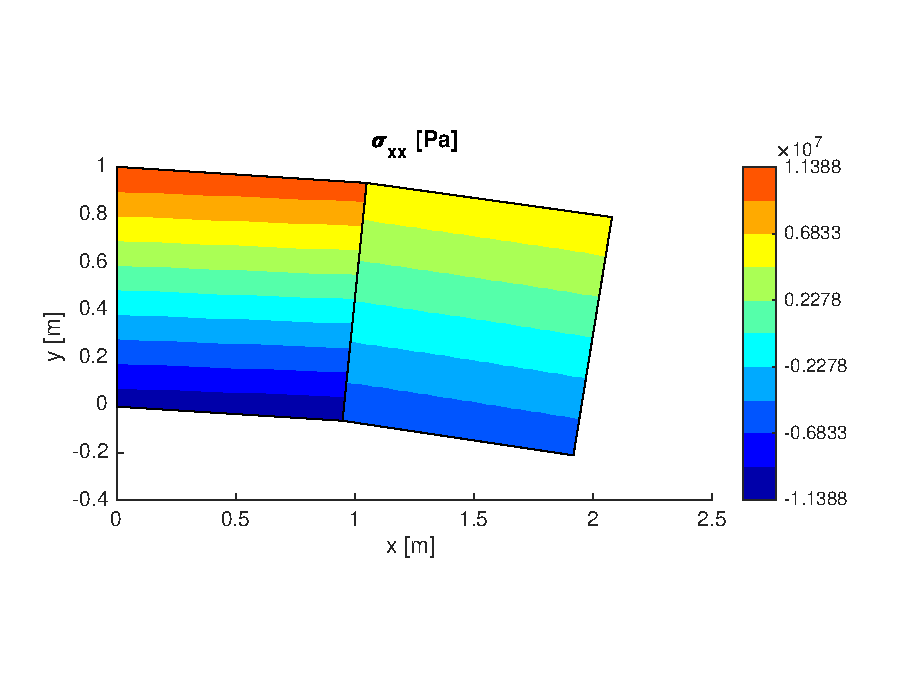
\includegraphics[width=0.5\textwidth]{code/q4domain.eps}
    \vspace{-1cm}
    \caption{Resultado de los códigos de la sección \ref{sec:q4codigo}. }
\end{figure}

\section*{Apuntes Auxiliares (Luis)}
Los elementos finitos siempre me dan soluciones más rígidas que la realidad porque estoy limitando sus nodos de movimientos mediante el uso de polinomios. En la realidad persisten funciones más complejas. Esto significa que el método de elementos finitos me aproxima la realidad por el lado más rígido, esto se tiene que tomar en cuenta!

\section*{Tablas}
\begin{table}[htb!]
	\begin{tabular}{>{$n=$}l<{ \vspace{10pt}}*{13}{c}}
		0 &&&&&&&1&&&&&&\\
		1 &&&&&&$x$&&$y$&&&&&\\
		2 &&&&&$x^2$&&$xy$&&$y^2$&&&&\\
		3 &&&&$x^3$&&$x^2y$&&$xy^2$&&$y^3$&&&\\
		4 &&&$x^4$&&$x^3y$&&$x^2y^2$&&$xy^3$&&$y^4$&&\\
		5 &&$x^5$&&$x^4y$&&$x^3y^2$&&$x^2y^3$&&$xy^4$&&$y^5$&\\
		6 &$x^6$&&$x^5y$&&$x^4y^2$&&$x^3y^3$&&$x^2y^4$&&$xy^5$&&$y^6$
	\end{tabular}
	\caption{El triangulo de pascal de orden $n=6$.}
\end{table}
\begin{table}[htb!]
	\centering
	\begin{tabular}{ll}
		\hline
		\multicolumn{2}{c}{Factor Corrección para $\nu\approx0,25$}                             \\ \hline
		Perfil                                                   & $k$                             \\ \hline
		Rectangular $\frac{h}{b}\gtrsim1$                        & $\frac{5}{6}$                   \\
		Rectangular $\frac{h}{b}=0,5$                            & $0,7961$                        \\
		Rectangular $\frac{h}{b}=0,25$                           & $0,6308$                        \\
		Circular                                                 & $\frac{9}{10}$                  \\
		Tubo de paredes delgadas circular                        & $\frac{1}{2}$                   \\
		\multicolumn{1}{c}{\multirow{2}{*}{Wide Flange doble T}} & $k_y\approx \frac{A_f}{1,2 A}$ \\
		\multicolumn{1}{c}{}                                     & $k_z\approx \frac{A_w}{ A}$  \\ \hline 
	\end{tabular}
	\caption{$A_w$ es el área del alma y $A_f$ es el área del ala.}
	\label{tab:kcorrectionfactor}
\end{table}

\section*{Expresiones útiles}
Operador derivada
\begin{itemize}
	\item Barra: $\partial x$
	\item Viga: $\dpartial{v}{x}$
	\item 2D: $\begin{bmatrix}
	\partial/\partial x & 0\\
	0 & \partial/\partial y \\
	\partial/\partial y & \partial/\partial x
	\end{bmatrix}$

\end{itemize}

\begin{align}
\sigma_{v}&=\sqrt{\sigma_{x}^2+\sigma_{y}^2+\sigma_{z}^2 - \sigma_x \sigma_y-\sigma_x\sigma_z -\sigma_y \sigma_z +3(\sigma_{xy}^2+\sigma_{xz}^2 +\sigma_{yz}^2)} \\
\sigma_{v}&=\sqrt{\tfrac{1}{2}\left[  (\sigma_{11}-\sigma_{22})^2+(\sigma_{11}-\sigma_{33})^2+(\sigma_{22}-\sigma_{33})^2\right] +3(\sigma_{12}^2+\sigma_{13}^2 +\sigma_{23}^2)}
\end{align}

\begin{equation}
\lambda = \frac{E \nu}{(1+\nu)(1-2\nu)} \qquad\quad \mu=G=\frac{E}{2(1+\nu)}
\end{equation}

\begin{equation}
\begin{bmatrix}
\sigma_{xx} \\
\sigma_{yy} \\
\sigma_{xy}
\end{bmatrix}
={\frac{E}{1-\nu^2}} 
\begin{bmatrix}
1 & \nu & 0 \\
\nu & 1 &0 \\
0 & 0 & \frac{1-\nu}{2}
\end{bmatrix}
\cdot
\begin{bmatrix}
\varepsilon_{xx} \\
\varepsilon_{yy} \\
2\varepsilon_{xy}
\end{bmatrix}
\end{equation}

\begin{equation}
\begin{bmatrix}
\sigma_{11} \\
\sigma_{22} \\
\sigma_{12}
\end{bmatrix}
={\frac{E}{(1+\nu)(1-2\nu)}} 
\begin{bmatrix}
1-\nu & \nu &0 \\
\nu &1-\nu& 0 \\
0 & 0 & \frac{1-2\nu}{2}
\end{bmatrix}
\cdot
\begin{bmatrix}
\varepsilon_{11} \\
\varepsilon_{22} \\
2\varepsilon_{12}
\end{bmatrix}
\end{equation}

\begin{equation}
\sigma_{n}=\frac{\sigma_{xx}+\sigma_{yy}}{2}+\left(\frac{\sigma_{xx}-\sigma_{yy}}{2}\right)\cos 2\theta +\tau_{xy}\sin 2\theta 
\end{equation}

\begin{equation}
\tau_{n}=-\left(\frac{\sigma_{xx}-\sigma_{yy}}{2}\right)\sin 2\theta +\tau_{xy}\cos 2\theta 
\end{equation}

\begin{equation}
I=\int^1_{-1} \phi(\xi) \di \xi \approx \phi(\xi_1) W_1+\phi(\xi_2) W_2 \ldots \phi(\xi_n) W_n
\end{equation}
\begin{equation}
I=\int^1_{-1} \int^1_{-1}\phi(\xi,\eta) \di \xi \di \eta\approx \sum_i \sum_j W_i W_j\phi(\xi,\eta) 
\end{equation}

Se suele requerir que $\eta\leq 0,05$


Formulación de elemento rígido RBE2:
\newcommand{\squareangles}{\vartheta}
\begin{align*}
g_u = u_{s}-u_{m}+L_{e}\versor{v}_{y}\,\left(\frac{\theta_{m}\,\sin\left(\sqrt{\squareangles}\right)}{\sqrt{\squareangles}}+\frac{\varphi_{m}\,\psi_{m}\,\left(\cos\left(\sqrt{\squareangles}\right)-1\right)}{\squareangles}\right)-&L_{e}\versor{v}_{z}\,\left(\frac{\psi_{m}\,\sin\left(\sqrt{\squareangles}\right)}{\sqrt{\squareangles}}-\frac{\varphi_{m}\,\theta_{m}\,\left(\cos\left(\sqrt{\squareangles}\right)-1\right)}{\squareangles}\right)\\
 - \frac{L_{e}\versor{v}_{x}\,\left({\psi_{m}}^2+{\theta_{m}}^2\right)\,\left(\cos\left(\sqrt{\squareangles}\right)-1\right)}{\squareangles}
\end{align*}

\begin{align*}
	g_v = v_{s}-v_{m}-L_{e}\versor{v}_{x}\,\left(\frac{\theta_{m}\,\sin\left(\sqrt{\squareangles}\right)}{\sqrt{\squareangles}}-\frac{\varphi_{m}\,\psi_{m}\,\left(\cos\left(\sqrt{\squareangles}\right)-1\right)}{\squareangles}\right)+&L_{e}\versor{v}_{z}\,\left(\frac{\varphi_{m}\,\sin\left(\sqrt{\squareangles}\right)}{\sqrt{\squareangles}}+\frac{\psi_{m}\,\theta_{m}\,\left(\cos\left(\sqrt{\squareangles}\right)-1\right)}{\squareangles}\right)\\ -\frac{L_{e}\versor{v}_{y}\,\left({\varphi_{m}}^2+{\theta_{m}}^2\right)\,\left(\cos\left(\sqrt{\squareangles}\right)-1\right)}{\squareangles}
\end{align*}

\begin{align*}
g_w = w_{s}-w_{m}+L_{e}\versor{v}_{x}\,\left(\frac{\psi_{m}\,\sin\left(\sqrt{\squareangles}\right)}{\sqrt{\squareangles}}+\frac{\varphi_{m}\,\theta_{m}\,\left(\cos\left(\sqrt{\squareangles}\right)-1\right)}{\squareangles}\right)-&L_{e}\versor{v}_{y}\,\left(\frac{\varphi_{m}\,\sin\left(\sqrt{\squareangles}\right)}{\sqrt{\squareangles}}-\frac{\psi_{m}\,\theta_{m}\,\left(\cos\left(\sqrt{\squareangles}\right)-1\right)}{\squareangles}\right) \\  - \frac{L_{e}\versor{v}_{z}\,\left(\cos\left(\sqrt{\squareangles}\right)-1\right)\,\left({\varphi_{m}}^2+{\psi_{m}}^2\right)}{\squareangles}
\end{align*}

donde \(\vartheta = \varphi_m^2 + \psi_m^2 + \theta_m^2\)


\begin{equation*}
	g_\varphi = \varphi_s - \varphi_m\, , \qquad g_\psi = \psi_s - \psi_m\, , \qquad g_\theta = \theta_s - \theta_m
\end{equation*}


En 2D


\clearpage
\section*{Figuras}
\begin{figure}[htb!]
	\centering
	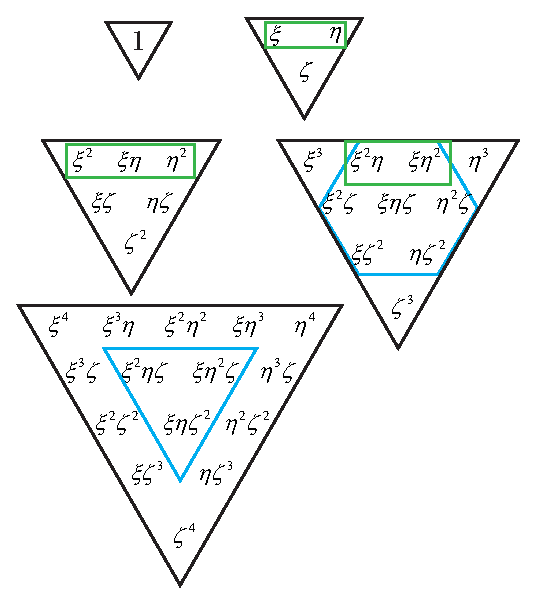
\includegraphics[width=0.5\textwidth]{fig/pascalsTetra.eps}
	\caption{El tetraedro de Pascal. Los términos de los elementos \textit{serendipidad} están encuadrados.}
	\label{fig:PascalsTetrahedron}
\end{figure}

\begin{figure}[htb!]
	\centering
	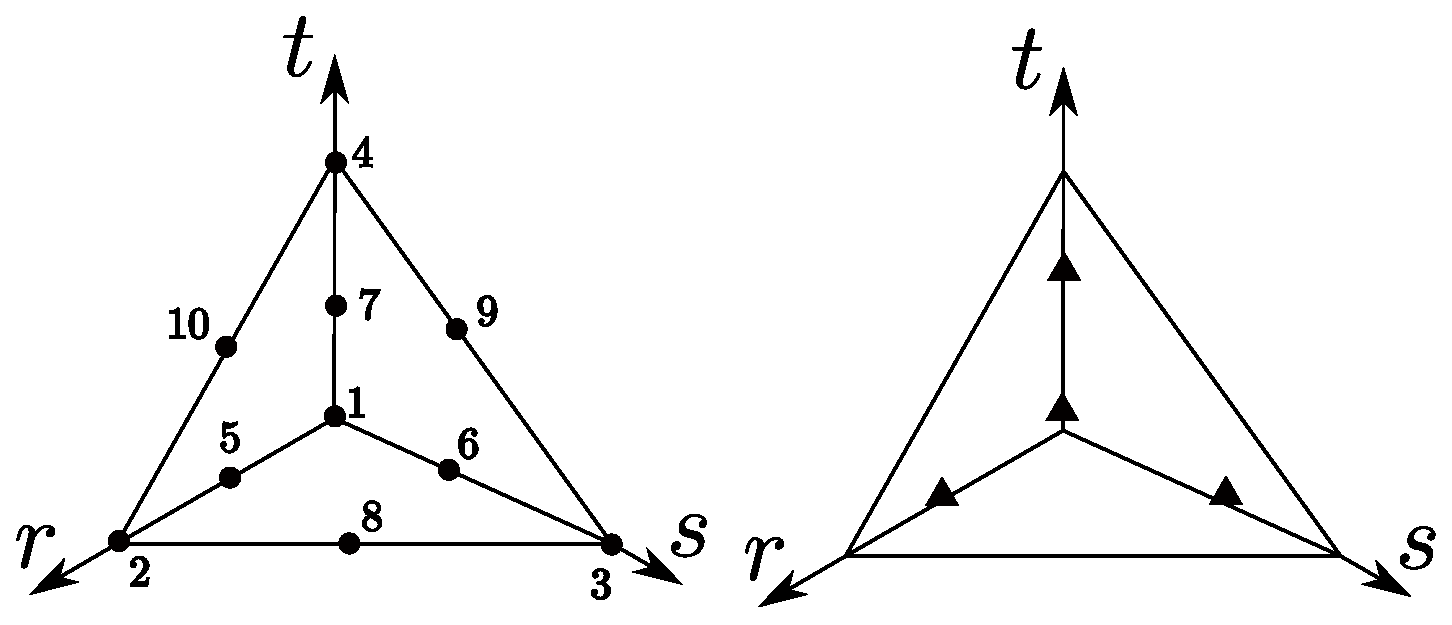
\includegraphics[width=0.8\textwidth]{fig/T10numbering.eps}
	\caption{Numeración de un tetraedro de diez nodos y la ubicación de los puntos Gauss para un grado de precisión 2.}
	\label{fig:T10numbering}
\end{figure}

%\clearpage

\input{\feaQP}
\input{\annexFile}
\clearpage
\bibliography{bibliografia} % Indica archivo

\end{document} 




% \begin{comment}
%     \section{Dudas}
%     \begin{enumerate}
%         \item Pg. 223 Cook: $\Mk$ de un solido 8 nodos se integra con $n=2$, pero $\MB$ se integra con $n=3$. Pero se necesita $\MB$ para obtener $\Mk$.
%         \item Si quiero verificar calidad de un elemento, me basta con pararme arriba cada punto Gauss y verificar que $\Djac$ no sea igual a cero y que no cambie de signo?
%         \item Tengo un problema plain strain pero tengo $q(x)$ en [N/m]. No lo integro con $t$! No? Inversamente, para el mismo problema, si tengo solo presiones o fzas volumetricas puedo olvidarme que existe $t$ y no usarla para el calculo de la matriz rigidez (y presiones/fzas vol). Se le dice singularidad a un punto donde $\Djac$ es cero
%         \item Si quiero tensiones en puntos Gauss, cambia la dimension de $\MB$ cuando itero sobre los puntos? Cook dice que $\MB$ is calculated from (lower order) displacement field. wtf?
%         \item \textbf{Follow-up} Cuando itero sobre los mismos Puntos de Gauss para obtener tensiones, cambian mis $\MN$? Sé que puedo usar los puntos de Gauss para extrapolar tensiones en los nodos, pero hablo antes de eso
%         \item Para un elemento me conviene siempre ser perfectamente simétrico en la elección del orden del polinomio? Hay alguna vez que voy a tomar $[1\ms x\ms y\ms xy\ms x^2]$ antes de tomar algo por el estilo de  $[1\ms x\ms y\ms y^2\ms x^2]$
%     \end{enumerate}
%     \end{comment}



Conceptos de modelado y de uso de software

Primer step, el modelo matematico. se representan las caracteristicas esenciales y lo
que se considera importante o relacionado al problema tratado, que pueden ser los detalles.

No necesariamente se tenga en cuenta el metodo de solucion al momento de modelado matematico
pero si sirve tener conocimiento de como funciona un FEA para saber cuanto detalle incluir.

Es importante conocer la teoria que se maneja y si aplica. Teoria de vigas supone material homogeneo y 
deflexiones pequeñas. Si se va de rango entonces te vas del rango donde es valida tu solucion.

Se recomienda que se empiece con un plan flexible que puede ser modificado a medida que se aprende mas del problema
que empezar de una con FEA. Planning requiere de 
*que resultados son los deseados, que se busca?
* Como serán verificados los resultados
* Hay una tendencia de aceptar los resultados del FEA de una por el tiempo que se invirtio en ellos,
esto se contraresta teniendo en mano los resultados aproximados ANTES de comenzar el FEA. 

*No se suelen usar elementos de deformacion constante porque no muestran la variacion lineal de la 
deformacion que aparece tan seguido en problemas con flexion y porque sufren de problemas numericos. 
(shear locking)

Thin walled sections!
Element Shape / Distribution!
